\chapter{Models for lagrangian injection}
	\label{ch4:sli_development}

\section{Introduction}

Chapter \ref{ch3:disperse_phase_methods} introduced numerical formalisms to represent dispersed two-phase flows. Special emphasis was given to the lagrangian representation of the fluid phase, as it is a widely employed approach in aerospace applications due to its low computational cost with respect to other formalisms and its ability to account for extra physics such as collisions, evaporation and combustion. The chapter culminated with the presentation of lagrangian models to model fuel injection in MSFI systems, giving extra attention to the state of the art in methodologies for simulating JICF. 

In this work, a novel numerical methodology to build numerical injectors for performing dispersed phase simulations in MSFI systems has been developed. The injectors built with this methodology have been baptised as Smart Lagrangian Injectors (SLI). Figure \ref{fig:state_art_injection} shows the location of the new method into the proposed classification of existing numerical models for lagrangian injection: SLI are built by learning a reference spray, which can be obtained either experimentally or numerically. In this thesis, the reference spray is obtained through resolved simulations of the atomization process. Computations performed with SLI will also account for the interaction of the dense liquid phase with the surrounding gas (blockage effect in liquid JICF) and secondary atomization models for further breakup of lagrangian particles.

This chapter details the underlying theory of SLI, showing all the key modeling ingredients. Section \ref{sec:ch4_spray_description} introduces mathematical foundations representing the spray which are used by describing the models in Section \ref{sec:ch4_models_flowchart}. The learning methodology to build injectors from a reference spray is defined in Section \ref{sec:ch4_SLI_learning}. Finally, the theory of the models blocks accounting for the blockage effect and secondary atomization models are discussed respectively in Sections \ref{sec:ch4_dense_core_modelling} and \ref{sec:ch4_secondary_atomization_modeling}.
 

%In this work, this new methodology has been applied to model liquid JICF injection, whose reference spray for the learning process has been obtained by performing resolved simulations of atomization with an academic test case. The results of these simulations are shown in Chapter \ref{ch5:jicf_resolved_simulations}. In a latter step, the SLI built from these simulations are applied to initialise dispersed phase computations for the same configuration in Chapter \ref{ch6:jicf_lgs_simulations}. Finally, all the methodology is applied in Part \ref{part3:BIMER} to a multipoint burner.



\section{Mathematical description of sprays}
	\label{sec:ch4_spray_description}

In $\S$\ref{subsec:ch3_statistical_methods}, dispersed sprays resulting from atomization were described by a function $f$ which represented the number density function of droplets. Then, all spray characteristics can be obtained by a proper definition and integration of $f$. Several methods targeting the determination of $f$ were discussed in Chapter \ref{ch3:disperse_phase_methods}, from statistical approaches to the LPP representation. Even if only statistical approaches make use of the WBE formulation, LPP can be considered as an approximation to the $f$ function by considering the point particle approximation. Consequently, since in this work the LPP representation is chosen to represent dispersed phase flows, a mathematical representation of dispersed sprays based on the function $f$ as given by Eq. (\ref{eq:f_spray_description_subramanian}) is used. This section intends to provide some theoretical foundations for the developed models from a generic, mathematical perspective. The rest of the chapter will be dedicated to explain how this formulation is applied in the current work. \\

\clearpage

\subsection{General formulation}

The spray produced by atomization can be described by a continuous function $F$:

\begin{equation}
F \left( t, \textbf{x}, \textbf{u}, D \right) 
\end{equation}

which is defined in the whole spatial domain $\Omega \left( \boldsymbol{x} \right)$, $\forall \boldsymbol{x} = \left\lbrace x, y, z \right\rbrace^T \in {R}^3$. In this first version of SLI, the spray will be characterized in plane surfaces. Therefore, it is of interest to sample the spray crossing a surface $\mathcal{S}$ belonging to the whole spatial domain: $\mathcal{S} \subset \Omega $. The spray sampled in this surface is described by a continuous function $f$:

\begin{equation}
\label{eq:f_general}
 f \left( t, \textbf{x}, \textbf{u}, D \right) = F \left( t, \textbf{x}, \textbf{u}, D \right) ~ \forall ~ \textbf{x} \in \mathcal{S}
\end{equation}

As $f$ is defined in a surface, it can be spatially represented by only two coordinates. These surface coordinates can be expressed as a vector $\boldsymbol{s} = \left\lbrace \xi, \eta \right\rbrace$. They can represent any type of surface, from cartesian to curvilinear. Therefore, the function $f$ can be expressed in terms of $\boldsymbol{s}$ as:

\begin{equation}
\label{eq:f_surface_coordinates}
f \left( t, \boldsymbol{s}, \textbf{u}, D \right)  
\end{equation}

Since both Eqs. (\ref{eq:f_general}) and (\ref{eq:f_surface_coordinates}) are identical, there is an equivalence between $\boldsymbol{x} = \left\lbrace x, y, z \right\rbrace$ and $\boldsymbol{s} = \left\lbrace \xi, \eta \right\rbrace$. This relation can be expressed mathematically as:

\begin{equation}
\label{eq:morphism_general_definition}
h : \boldsymbol{x} \rightarrow \boldsymbol{s}
\end{equation}

% Cool about morphisms: https://www.euclideanspace.com/maths/discrete/structure/map/morphism/index.htm

where $h$ is a mapping function, or morphism, that will transform from cartesian coordinates $\boldsymbol{x}$ to surface coordinates $\boldsymbol{s}$. \\


In this work, the variation of the spray characteristics with time will not be considered. Instead, the obtention and study of a stationary, mean spray will be the main objective of SLI. For such purpose, the spray will be sampled in time for a period $T$ which should be large enough in order to obtain a converged spray (see $\S$\ref{subsec:SLI_spray_convergence}), hence eliminating the dependence with time. Mathematically speaking, this can be represented through integration:

\begin{equation}
\label{eq:f_general_time_integrated}
f \left( \boldsymbol{s}, \boldsymbol{u}, D \right) = \frac{1}{T} \int_0^T f \left( t, \boldsymbol{s}, \boldsymbol{u}, \right) dt
\end{equation}

Eventually, for a better characterization of the spray, the sampling surface $\mathcal{S}$ will be spatially discretized into several elements, or probes, of size $\Delta S$. In this way, the spray within each probe can be independently study to provide \textbf{spatially refined statistics}. The representation of spatially refined statistics can be obtained from $f$ by integrating spatially this function within each probe with center $\left( \xi_\mathrm{j}, \eta_\mathrm{k} \right)$:

\begin{equation}
\label{eg:f_discrete}
f_\mathrm{j,k} \left( \boldsymbol{s}_\mathrm{j,k}, \boldsymbol{u}, D \right) = \frac{1}{\Delta \xi \Delta \eta} \int_{\xi_\mathrm{j-1/2}}^{\xi_\mathrm{j+1/2}} \int_{\eta_\mathrm{k-1/2}}^{\eta_\mathrm{k+1/2}}  f \left( \boldsymbol{s}, D \right) d\xi d\eta
\end{equation}

\subsection{Spray formulation in jet in crossflow}

A more precise, less abstract interpretation for the SLI spray formulation can be obtained by applying the general formulation to a liquid JICF problem, atomication case introduced in $\S$\ref{sec:ch1_fuel_injection_technology}. Figure \ref{fig:JICF_spray_formulation} shows a liquid JICF from a resolved atomization simulation. As observed, the liquid leaves the injection nozzle as a coherent jet moving along the $z$ direction and then starts bending towards the $x$ direction. Atomization starts taking place and breaks the jet into firstly ligaments and, subsequently, droplets. The resulting droplets from the atomization process conform a spray that can be analyzed by the SLI strategy. Therefore, to study this spray, first droplets need to be sampled in sampling surfaces. In a geometrically simple JICF problem as the one from Figure \ref{fig:JICF_spray_formulation}, the sampling surfaces are planes perpendicular to the crossflow direction $x$ denoted in the figure by $S$. The surface coordinates $\boldsymbol{s}$ aforementioned correspond therefore to the in-plane coordinates in the sampling surface, which in the system of reference depicted in Figure \ref{fig:JICF_spray_formulation} yield $\boldsymbol{s} = \left\lbrace y, z \right\rbrace$. Therefore the discrete, spatially refined statistics are obtained in probes centered at $\left( y_\mathrm{j}, z_\mathrm{k} \right)$, and the function $f_\mathrm{j,k}$ given generally by Eq. (\ref{eg:f_discrete}) can be applied to the proposed JICF formulation as:

\begin{equation}
\label{eg:f_discrete_jicf}
f_\mathrm{j,k} \left( \boldsymbol{s}_\mathrm{j,k}, \boldsymbol{u}, D \right) = \frac{1}{\Delta y \Delta z} \int_{y_\mathrm{j-1/2}}^{y_\mathrm{j+1/2}} \int_{z_\mathrm{k-1/2}}^{z_\mathrm{k+1/2}}  f \left( \boldsymbol{s}, \boldsymbol{u}, D \right) dy dz
\end{equation}

\begin{figure}[h!]	
	\centering
	\includeinkscape[inkscapelatex=false,scale=0.6]{./part2_developments/figures_ch4_SLI/JICF_spray_formulation}
	\caption{Illustration of SLI spray formulation in a liquid JICF.}
	\label{fig:JICF_spray_formulation}
\end{figure}


\section{Models for lagrangian injection}
	\label{sec:ch4_models_flowchart}
	
The objective of the models 	for performing lagrangian injection is to provide the necessary input parameters to initialize disperse-phase simulations. These input parameters are intended to represent a realistic spray resulting from primary atomization. Most existing models perform lagrangian injection by neglecting the atomization process due to its complexity, while other rely on experimental data or correlations which are valid for a limiting range of operating conditions (see $\S$\ref{sec:ch3_state_art_lagrangian_injection} for a discussion on the state of the art in dispersed-phase simulations of MSFI systems). 

With this objective in mind and knowing the limitations of the existing approaches, the intention of this work is to develop models that can be fed from primary atomization data to: 1) inject a proper dispersed-phase and 2) model as accurately as possible the momentum exchange due to the liquid-gas interaction in the primary atomization region. The second point has often been neglected in many dispersed phase simulations, and has been the object of multiple studies dealing with primary atomization. To address both points, this thesis relies firstly on \textbf{numerical simulations of the resolved atomization process} using an ACLS/AMR approach ($\S$\ref{subsec:ch2_ACLS}). These simulations are used to construct a spray database by sampling the droplets passing through planes perpendicular to the crossflow direction and then applying the spray formulation previously presented. The functions $f \left( \boldsymbol{s}, \boldsymbol{u}, D \right) $ of the spray formulation represent therefore the statistical distributions of the spray's size, velocity and fluxes that are processed in a \textbf{lagrangian injectors learning process} to eventually yield the discretized spray $f_\mathrm{j,k} \left( \boldsymbol{s}_\mathrm{j,k}, \boldsymbol{u}, D \right)$ that is used as lagrangian injector to initialize \textbf{dispersed-phase simulations}. At the same time, the liquid-gas interaction between the jet dense core and the crossflow is also analyzed and learnt to provide a model that contributes to the liquid-gas \textbf{momentum exchange} in the disperse-phase simulations, which a priori is neglected (and which many models do not take into account or circumvent by introducing experimental correlations). In this way, the full methodology currently relies only on the data from the resolved atomization simulations in order to fully initialize dispersed-phase computations. Therefore, any operating point could be simulated through resolved simulations and learnt with the proposed methodology without the need of relying on experimental data or semi-empirical correlations. The proposed approach will be called hereafter as Smart Lagrangian Injectors (SLI).

The full approach of SLI is detailed schematically in the flowchart of Figure \ref{fig:SLI_graphic_description}. The process is summarized in the following lines:


\begin{enumerate}

	\item \textbf{Resolved atomization simulations} are performed to build a spray (statistical spray distributions) and liquid-gas interaction (momentum exchange) database (Chapter \ref{ch5:jicf_resolved_simulations}).
	
	\item This database is used and processed by the models to \textbf{learn the spray state} and build lagrangian injectors (Chapter \ref{ch4:sli_development}). The learning part consists of the following parts: \textbf{spray sampling} ($\S$\ref{subsec:SLI_spray_sampling}), \textbf{spatial discretization} ($\S$\ref{subsec:SLI_spatial_discretization}) and \textbf{spray convergence} ($\S$\ref{subsec:SLI_spray_convergence}) of the injectors. The convergence can be checked either globally in the sampling plane, or locally by dealing with the sprays contained in each discrete, individual probe in order to perform a \textbf{converge-driven classification} ($\S$\ref{subsec:SLI_quadtrees_discretization}).
	
	\item \textbf{Dispersed-phase simulations} are initialized with the injectors developed with this methodology (Chapter \ref{ch6:jicf_lgs_simulations}). Apart from the lagrangian injectors that inject the liquid phase, the two following submodels are also contained in these simulations: 
	
		\begin{itemize}
	
		\item \textbf{Dense core learning} with the \textbf{actuator line model} in order to take into account the perturbation effect of the liquid dense structures (i.e. the liquid dense core in the JICF) in the gaseous phase during lagrangian simulations ($\S$\ref{sec:ch4_dense_core_modelling}). The information to characterize the dense core is taken from the resolved simulations and later imposed into lagrangian ones.
		
		\item \textbf{Secondary atomization models} to consider further possible breakup of spherical droplets during lagrangian simulations ($\S$\ref{subsec:SLI_spatial_discretization}).
		
		\end{itemize}


\end{enumerate}


\begin{figure}[h!]	
	\centering
	\includeinkscape[inkscapelatex=false,scale=0.3]{./part2_developments/figures_ch4_SLI/SLI_graphic_description_with_learning_boxes}
	\caption{Flowchart of the SLI formulation applied to liquid JICF.}
	\label{fig:SLI_graphic_description}
\end{figure}


%
%\section{Models for lagrangian injection (OLD)}
%	\label{sec:ch4_models_flowchart}


%\begin{figure}[h!]	
%	\centering
%	\includeinkscape[inkscapelatex=false,scale=0.3]{./part2_developments/figures_ch4_SLI/SLI_graphic_description}
%	\caption{Illustration of SLI working principle \textbf{CHANGE FIGURE TO NEW CONFIG WITHOUT SIDE WALLS}.}
%	\label{fig:SLI_graphic_description}
%\end{figure}




%\begin{figure}[h!]	
%	\centering
%	\includeinkscape[inkscapelatex=false,width=17cm]{./part2_developments/figures_ch4_SLI/SLI_flowchart_with_pictures}
%	\caption{Flowchart for proposed models of lagrangian injection.}
%	\label{fig:SLI_flowchart}
%\end{figure}




\section{Lagrangian injectors learning}
	\label{sec:ch4_SLI_learning}


\subsection{Spray sampling}
\label{subsec:SLI_spray_sampling}

\subsubsection*{Identification of liquid structures in resolved simulations}

The first step in the learning process is to obtain the spray from resolved atomization simulations. For this purpose, droplets must be identified in space. According to the ACLS methodology ($\S$\ref{subsec:ch2_ACLS}), liquid regions are identified by level set values $\psi > 0.5$, and the interface $\Gamma$ is located at $\psi = 0.5$. It is possible then to identify and tag individual liquid structures as independent closed regions of $\Gamma$, whose domain is denoted as $\Omega_l$. Each structure can then be characterized by its volume $V_\mathrm{dr}$, its center of mass location $\textbf{x}_\mathrm{dr}$ and velocity $\textbf{u}_\mathrm{dr}$, and maximum and minimum distances from the interface to the center of mass $R_\mathrm{max}$ and $R_\mathrm{min}$, as depicted in Figure \ref{fig:droplet_sampling_parameters}. The formulas used for calculating these parameters are shown in Table \ref{tab:sampling_parameters}. 

\begin{table}[!h]
\centering
\caption{Parameters sampled from resolved atomization simulation}
\begin{tabular}{ccl}
\thickhline
Parameter & Definition & Description \\
\thickhline
$V_\mathrm{dr}$ & $\displaystyle \int_{\Omega_l} d V$ & Volume enclosed by interface  \\
\hline
$\textbf{x}_\mathrm{dr}$ & $\displaystyle \frac{1}{V} \int_{\Omega_l} \boldsymbol{x} d V$ &   Location of center of mass \\
\hline
$\textbf{u}_\mathrm{dr}$ & $\displaystyle \frac{1}{V} \int_{\Omega_l} \textbf{u} \left( \boldsymbol{x} \right) d V$ & Velocity of center of mass  \\
\hline
$r_\mathrm{max}$ & $\displaystyle \max \left( | \textbf{x} - \textbf{x}_\mathrm{dr} | \right) \forall \textbf{x} \in \Omega_l$ & Maximum distance to center of mass \\
\hline
$r_\mathrm{min}$ & $\displaystyle \min \left( | \textbf{x} - \textbf{x}_\mathrm{dr} |  \right) \forall \textbf{x} \in \Omega_l$ & Minimum distance to center of mass \\
\thickhline
\end{tabular}
\label{tab:sampling_parameters}
\end{table}

\begin{figure}[h!]	
	\centering
	\includeinkscape[inkscapelatex=false,scale=0.5]{./part2_developments/figures_ch4_SLI/droplet_sampling_parameters}
	\caption{Parameters characterizing liquid structures sampled in resolved atomization simulations. }
	\label{fig:droplet_sampling_parameters}
\end{figure}

In order to get statistics for spray characterization, it is useful to define a characteristic size of each liquid structure. For this purpose, an equivalent radius $r_\mathrm{dr}$ is calculated from the liquid volume $V_\mathrm{dr}$:

\begin{equation}
\label{eq:ch4_r_equivalent_calculation}
r_\mathrm{dr} = \sqrt[3]{\frac{3 V_\mathrm{dr}}{4 \pi}}
\end{equation}

which is the radius of a sphere containing the same volume as the liquid structure. The equivalent diameter is then $d_\mathrm{dr} = 2 r_\mathrm{dr}$. In cases where sampled structures are spherical droplets, $R_\mathrm{dr}$ is the true radius and, therefore, a representative measure of the droplets' size. On the other hand, if liquid structures are not fully spherical (which is often the case after primary atomization), the equivalent radius does not provide full information on their topology. To determine the deviation of the identified liquid structure from a sphere, the radii $r_\mathrm{max}$ and $r_\mathrm{min}$ can be used to calculate the deformation parameters $\alpha$ and $\beta$ \citepColor[zuzio_improved_2018]:

\begin{equation}
\label{eq:ch4_deformation_parameters_alpha_beta_calculation}
\alpha = \frac{r_\mathrm{max}}{r_\mathrm{dr}} ~~ ; ~~ \beta = \frac{r_\mathrm{min}}{r_\mathrm{dr}}
\end{equation}	

By definition, $\alpha \geq 1$ and $\beta \leq 1$. A perfect sphere would present $\alpha = \beta = 1$.

In this work, no distinction between droplets and ligaments has been done to construct the injectors after the learning procedure. Hence, hereafter all liquid structures will be referred as droplets, and the term droplet sampling will be used. Inclusion of distinction between ligaments and droplets (i.e. between non-spherical and spherical structures) could be further taken into account with parameters $\alpha$ and $\beta$ to, for example, modify drag coefficients in lagrangian simulations at the first steps after injection \citepColor[bagheri_drag_2016]. 


\subsubsection*{Sampling procedure}

Droplets are sampled according to their center of mass (CM) location. Note that, despite the ACLS methodology being eulerian, liquid structures produced by resolved simulations are being tracked as lagrangian particles (lagrangian tracking). Two sampling methods based on experimental techniques can be used \citepColor[tropea_optical_2011], their main difference being the topology of the sampling regions (see Figure \ref{fig:tropea_droplet_sampling}):

\begin{itemize}

	\item A control volume (unit volume in Figure \ref{fig:tropea_droplet_sampling}) can be defined where particles contained inside are sampled at a particular time instant. This method produces a \textbf{volume distribution}. 
	
	\item A surface area (unit area in Figure \ref{fig:tropea_droplet_sampling}) or plane where droplets crossing it during a given time are sampled. A \textbf{flux density distribution} is obtained in this case.

\end{itemize}


\begin{figure}[h!]
	\centering
	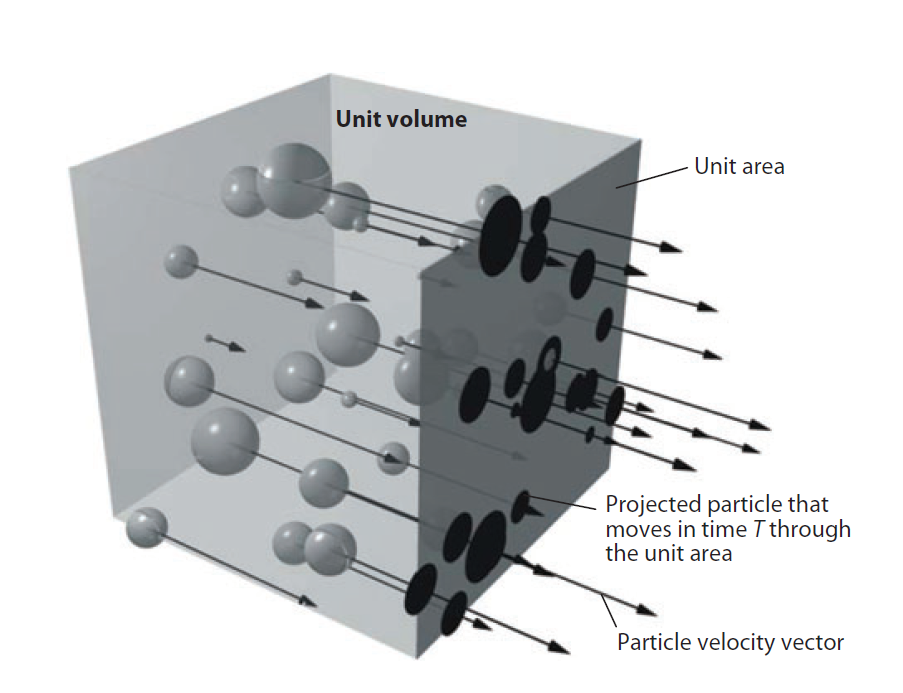
\includegraphics[scale=0.6]{./part2_developments/figures_ch4_SLI/tropea_droplet_sampling}
	\caption{Droplet sampling prodecure. Source: \citeColor[tropea_optical_2011]}
	\label{fig:tropea_droplet_sampling}
\end{figure}

In this work, droplets crossing surface areas are sampled, hence obtaining flux density distributions. This method is chosen to be closer to experimental measurements performed in jet in crossflow configurations \citemColor[wu_spray_1998,becker_breakup_2002]. The defined surface areas employed will be hereafter referred as \textbf{sampling planes}. To determine when a droplet is sampled, a sampling rate $T_\mathrm{sample}$ is specified so that the current location and velocities of droplets CM at time $t$ is checked. Then, the location of each droplet at time $t + T_\mathrm{sample}$ is estimated by projecting the position of the center of mass with the current velocities. Droplets whose current location at $t$ and projected location at $t + T_\mathrm{sample}$ is at different sides of a sampling plane are sampled. This procedure is referred as \textbf{lagrangian projection} of droplets. It is computationally cheap, so can be performed in the resolved and dispersed phase computations without highly increasing the cost of the simulations. On the other hand, it has the main disadvantages that: 1) some actual crossing droplets might not be sampled and 2) contrarily, some droplets might be sampled twice. These downcomes of the methodology could be circumvented by including a tag field in the resolved simulations where droplets are assigned an ID number that does not change with time. However, this is not available yet and is difficult to implement, since the atomization process hinders droplet tagging as liquid structures change constantly during primary and secondary breakup.

The sampling rate is chosen so that that all droplets crossing the plane are collected. Droplets are accumulated with time, and then statistics are calculated. Choosing a right sampling rate ensures that at the end of the accumulation process, the mass flow rate in average is the actual rate passing through the sampling plane in the resolved simulations. If the sampling rate is too low, some droplets might be missed and the flow rate captured will not be the right one (aliasing phenomenon on the spray sampling procedure). Another technique to measure flow rates directly in resolved atomization simulations, called interior boundaries, has been developed in this thesis. This one is later explained in $\S$\ref{subsec:ch5_interior_boundaries} and compared to the rates obtained from the lagrangian tracking procedure in $\S$\ref{subsec:ch5_sli_fluxes_vs_IBs}. \\

\subsubsection*{Defining statistics for sprays}

The resulting accumulated spray is composed of a polydisperse ensemble of droplets, each droplet characterized by parameters from Table \ref{tab:sampling_parameters}. In order to characterize the spray, it is useful to define averaged and Root-Mean Squared (RMS) values for the whole spray from the individual droplets parameters. For an arbitraty magnitude $f$, the arithmetic mean and RMS values would be defined as follows:

\begin{equation}
\label{eq:ch4_f_arbitrary_mean_RMS_definition}
\overline{f} = \frac{1}{N_\mathrm{dr}} \sum_{i=1}^{N_\mathrm{dr}} f_i  ~~~~~~ ; ~~~~~~ f_\mathrm{RMS} = \sqrt{\overline{f^2} - \overline{f}^2}
\end{equation}

%\begin{equation}
%\overline{f} = \frac{1}{T} \sum f_i \Delta t_i ~~~~~~ ; ~~~~~~ f_\mathrm{RMS} = \sqrt{\overline{f^2} - \overline{f}^2}
%\end{equation}

where $N_\mathrm{dr}$ is the number of accumulated droplets. In the case of polydisperse sprays, where there are several liquid structures with different volumes, it is also useful to define volume-weighted averages in order to give more relevance to the properties of larger droplets. For an arbitrary magnitude $f$, the volume-weighted mean and RMS can be defined as:

\begin{equation}
\label{eq:ch4_f_arbitrary_mean_RMS_VW_definition}
\displaystyle \overline{f}_\mathrm{VW} = \frac{1}{\sum_{i=1}^{N_\mathrm{dr}} V_i} \sum_{i=1}^{N_\mathrm{dr}} f_i V_i ~~~~ ; ~~~~ f_\mathrm{RMS,VW} = \sqrt{\displaystyle \overline{f^2 }_\mathrm{VW} - \displaystyle \overline{f }_\mathrm{VW}^2}
\end{equation}

where $V_i$ is the volume of each liquid structure. Related to the injectors the definition of mean and RMS values, either arithmetic or weighted-averaged, will be applied to the velocities in the three directions, $\alpha$ and $\beta$. \\

In two-phase flow problems involving disperse-phase sprays, it is useful to define average diameters of droplets with definitions different than the one given by applying Eq. (\ref{eq:ch4_f_arbitrary_mean_RMS_definition}). since they are better representative of the physical problems involving mass or heat transfer \citepColor[lefebvre_atomization_2017]. For combustion applications, the most used averaged diameter is the Sauter Mean Diameter (SMD):

\begin{equation}
\label{eq:ch4_SMD_definition}
\mathrm{SMD} = \frac{\sum_{i=1}^{N_\mathrm{dr}} d_i^3 }{\sum_{i=1}^{N_\mathrm{dr}} d_i^2}
\end{equation} 

where $d_i$ is the individual diameter of each droplet. The numerator of this expression is proportional to the cube of the diameter, which is equivalent to the droplet volume. The denominator is dependent to its square, which is related to the droplet liquid surface. Therefore, the SMD represents the relation between the liquid volume and surface in a spray. This is specially useful when evaporation is present (i.e. prior to combustion), since evaporation occurs when the specific liquid surface (the surface of liquid in contact with air) is large: that is, when the SMD is small.

Finally, a last useful magnitude that can be defined for a convecting spray is the liquid flow rate, which is a mean quantity by definition. Considering a sampling surface as in Figure \ref{fig:tropea_droplet_sampling}, the mean liquid flow rate passing through it can be obtained as:

\begin{equation}
\label{eq:ch4_Ql_definition}
Q_l = \frac{d V_l}{dt} \approx \frac{\Delta V_l}{\Delta t} = \frac{\sum_{i=1}^{N_\mathrm{dr}} V_i}{t_\mathrm{acc}} 
\end{equation}

where $t_\mathrm{acc}$ is the total accumulation time. $Q_l$ yields an absolute flux that represents the mass flux passing through each sampling plane considered. If the sampling plane is discretized in several probes (see $\S$\ref{subsec:SLI_spatial_discretization}) and the fluxes are determined within them, the addition of all probes' fluxes will yield the absolute flux from the whole sampling plane. In these cases, the fluxes from each probe will depend on the probes surface $S_\mathrm{probe}$: the smaller $S_\mathrm{probe}$, the smaller the absolute flux. Therefore, when dealing with spatially discretized sprays it is useful to express the absolute flux in relation $S_\mathrm{probe}$. This yields a surface-weight flux $q_l$, named also volume flux:

\begin{equation}
\label{eq:ch4_volume_flux_definition}
q_l = \frac{Q_{l,\mathrm{probe}}}{S_\mathrm{probe}}
\end{equation}

The value of $q_l$ converges with the probe size, as opposed to $Q_l$. Effectively, if the size of the probe $\Delta y \times \Delta z$ is reduced, the liquid flux as defined by Eq. (\ref{eq:ch4_Ql_definition}) will also decrease since less droplets might be sampled in a smaller surface. Nevertheless, the volume flux $q_l$ defined by Eq. (\ref{eq:ch4_volume_flux_definition}) will we maintaned because, despite the reduction in $Q_l$, the probe surface is also smaller.

\clearpage

%The in-plane, accumulated spray is discretized with a grid composed of uniform probes with surface $S_\mathrm{probe}$. For each probe, a surface-weight flux can be calculated. Denoted as $q_l$, it can be obtained as:
%
%\begin{equation}
%\label{eq:ch4_Ql_definition}
%q_l = \frac{Q_l}{S_\mathrm{probe}}
%\end{equation}

%The advantage of $q_l$ is that it converges with the probe size, as opposed to $q_l$. Effectively, if the size of the grid $\Delta y$ x $\Delta z$ is reduced, the liquid flux as defined by Eq. (\ref{eq:ch4_Ql_definition}) will also decrease since less droplets might be sampled in a smaller surface. Nevertheless, the volume flux $q_l$ will we maintaned because, despite the reduction in $Q_l$, the probe surface is also smaller.



\subsection{Spray convergence}
\label{subsec:SLI_spray_convergence}

Simulations using the ACLS/AMR methodology resolve atomization and provide deep insight on the driving physical phenomena. Nevertheless, their main limitation is their cost (see $\S$\ref{subsec:ch5_computational_performances}), which increases when more liquid is present in the domain. Consequently, the accumulation time of droplets will be finite and, logically, restricted to the physical time simulated. This can pose a problem for spray characterization, since statistics might not be converged if the number of sampled droplets is not sufficient.

Here, a methodology to evaluate spray convergence is proposed. The objective is to provide a quantitative measure to assess whether enough droplets have been sampled to obtain reliable statistics \citepColor[vie_particle-laden_2016]. If the spray is converged, then it can be spatially discretized to get local statistics that will conform the injectors ($\S$\ref{subsec:SLI_spatial_discretization}). This convergence criterion is also used to propose another discretization strategy in which refinement is performed following a quadtrees structure (convergence-driven discretization, see $\S$\ref{subsec:SLI_quadtrees_discretization}).

At each time step $t_i$ of the accumulation process, the spray will be formed by a number of droplets $N_{\mathrm{dr},i}$. This number will increase as more particles are accumulated with time, since all droplets sampled previously are also accounted for (hence the name accumulation). One can see this methodology as obtaining a \textbf{time-averaged spray}, since dependence with time is neglected. Statistics representing the spray, such as droplet size histograms, can be calculated on the accumulated spray at each time $t_i$. Figure \ref{fig:spray_convergence_description_accumulation_and_MSE_comparison} left shows an illustrated view of the size histogram evolution at several accumulation instants. The histogram indicates thes probability $f \left( d_\mathrm{dr} \right)$ of finding a droplet of size $d_\mathrm{dr}$ within a class $n$: $d_\mathrm{dr} \in \left[ d_{\mathrm{dr},n}-\Delta d_\mathrm{dr}/2, d_{\mathrm{dr},n}+\Delta d_\mathrm{dr}/2 \right]$. Its shape will change with accumulation time until an instant from which it will stay constant if more droplets are sampled. At this point, the spray will be considered to be converged. 

\begin{figure}[ht]
     \centering
     \begin{subfigure}[b]{0.45\textwidth}
         \centering
         \includeinkscape[inkscapelatex=true,scale=0.35]{./part2_developments/figures_ch4_SLI/size_distribution_evolution_with_accumulation}
     \end{subfigure}
     %\hfill
     \begin{subfigure}[b]{0.45\textwidth}
         \centering
          \includeinkscape[inkscapelatex=true,scale=0.45]{./part2_developments/figures_ch4_SLI/size_distribution_histograms_comparison}
     \end{subfigure}
        \caption{\textsl{Left}: Size histogram evolution with accumulation time of droplets. \textsl{Right}: comparison of two droplet size histograms from two consecutive time instants.}
	% See: https://stackoverflow.com/questions/35210337/can-i-plot-several-histograms-in-3d/35225919
        \label{fig:spray_convergence_description_accumulation_and_MSE_comparison}
\end{figure}



The main issue now is to determine quantitatively when the spray is converged. For this purpose, the histograms are compared in pairs at subsequent time instants, $t_i$ and $t_{i-1}$, as shown in Figure \ref{fig:spray_convergence_description_accumulation_and_MSE_comparison} right. The same number and width of droplets classes are used in both histograms. The difference between both histograms is then measured by means of a Mean Squared Error (MSE) function defined as:

\begin{equation}
\label{eq:MSE_definition}
MSE^{t_i} = \frac{1}{N} \sum_{n=1}^N \left( f_n^{t_{i-1}} - f_n^{t_i}  \right)^2
\end{equation}

where $N$ is the total number of classes in the histogram. This criterion is similar to the Cramer-von Mises measure to compare two statistical distributions \citepColor[anderson_distribution_1962]. The MSE can then be calculated at each accumulation time instant and then be normalized by the maximum value obtained, yielding a Normalized Mean Squared Error (NMSE) \citepColor[hanna_flacs_2004]:

\begin{equation}
NMSE^{t_i} = \frac{MSE^{t_i}}{\max_{t_i} \left( MSE \right)}
\end{equation}

The evolution of NMSE can be displayed with time as shown in Figure \ref{fig:NMSE_evolution}. The NMSE decreases with accumulation time until reaching a plateau, where the NMSE does not move significantly. Convergence is achieved at the beginning of this plateau, which is defined for values of the NMSE below a threshold $\varepsilon_\mathrm{th}$.

\begin{equation}
\label{eq:NMSE_convergence_criterion}
NMSE < \varepsilon_\mathrm{th}
\end{equation}

where $\varepsilon_\mathrm{th}$ is set to $0.03$ (i.e. $3 \%$).

%An additional criterion for convergence is added, which is the variation of the NMSE in the last 10 iterations. Hence, statistical convergence of the spray makes use of the following two criteria:
%
%\begin{itemize}
%
%	\item NMSE must be below $\varepsilon_\mathrm{th}$, as shown in the previous equation.
%	
%	\item In the last 10 iterations, the NMSE must be decreasing and lower to $\varepsilon_\mathrm{th}$.
%
%\end{itemize}




\begin{figure}[h!]
	\centering
	\includegraphics[scale=0.15]{./part2_developments/figures_ch4_SLI/spray_convergence_with_text.eps}
	\caption[Evolution of Normalized Mean Squared Error (NMSE) with respect to spray accumulation time.]{Evolution of Normalized Mean Squared Error (NMSE) with respect to spray accumulation time (solid line). The dashed line indicates the chosen threshold of $\varepsilon_\mathrm{th} = 3 \%$.}
	\label{fig:NMSE_evolution}
\end{figure}



It is worth noting that the convergence criterion based on NMSE introduced in this section depends solely on the equivalent droplets size $d_\mathrm{dr}$. Future work would include to extend this criterion to other magnitudes fundamental for a proper spray representation, such as velocities and flow rates. Furthermore, a time-independent spray has been considered in all the previous process by accumulating droplets and calculating statistics which do not depend on the time in which they were sampled. A perspective in this respect would be to obtain a transient spray in order to create unsteady numerical injectors. This could be useful in systems where thermoacoustic instabilities appear and there are fluctuations in the injected flow rates, such as aeronautical gas turbines \citepColor[lieuwen_unsteady_2012]. Further possible improvements could also include the use of information theory techniques for characterizing the convergence state, which have recently been applied and evaluated in sprays \citemColor[panao_assessment_2012,panao_statistical_2020].


%\subsubsection*{Old formulation}
%
%
%A Mean Squared Error (MSE) function is used:
%
%\begin{equation}
%MSE = \frac{1}{n} \sum_{i=1}^n \left( P_{N_{\mathrm{dr},2}} - P_{N_{\mathrm{dr},1}} \right)^2
%\end{equation}

\subsection{Spatial discretization of sprays}
\label{subsec:SLI_spatial_discretization}

Once the global accumulated spray at the sampling plane is converged, enough droplets have been sampled to perform a spatial discretization of the spray. The objective is to classify spatially the in-plane accumulated droplets into a grid composed of several rectangular probes so that spray statistics can be calculated within each probe individually. Later on each probe will conform an injector for the dispersed-phase simulations: the SLI is therefore the whole grid composed of all the discrete injectors.

Figure \ref{fig:SLI_discretization} shows an example of a discrete spray grid resulting from the spatial discretization process. The grid has dimensions ($w_\mathrm{spray}$, $h_\mathrm{spray}$), which correspond to its width and height given in the $y$ and $z$ directions respectively. Grid's dimensions can be calculated in three ways: 1) they can be chosen ad-hoc by the user (as long as they englobe the full spray in order not to miss sampled mass); 2) they are calculated automatically as given by the furthest droplets in the $y$, $z$ directions; 3) they are calculated automatically if the individual probe dimensions ($w_\mathrm{inj}$, $h_\mathrm{inj}$) are given by the user, in which case the grid size will be calculated accordingly in order to englobe the whole in-plane spray. The sketch at the right in Figure \ref{fig:SLI_discretization} shows a magnified view of a single probe of the grid, which composes an individual injector. The probe consists of dimensions ($w_\mathrm{inj}$, $h_\mathrm{inj}$) and center $x_\mathrm{inj}$. Each droplet in the probe is characterized by the parameters from Table \ref{tab:sampling_parameters}, from which the equivalent droplet diameter $d_\mathrm{dr}$ is calculated with Eq. (\ref{eq:ch4_r_equivalent_calculation}) and the deformation parameters $\alpha$ and $\beta$ with Eq. (\ref{eq:ch4_deformation_parameters_alpha_beta_calculation}). These parameters are then used to calculate statistics on each probe's spray, which are later used to perform injection. The parameters conforming each injector are later introduced in $\S$\ref{subsec:ch4_injectors_definition}. The spatially distributed statistics in the sampling grid can be represented in maps of mean and RMS values, which give an idea of the spray shape in terms of diameters, fluxes and velocity distributions. Examples of maps for the resolved simulations of liquid JICF cases are shown later in Chapters \ref{ch5:jicf_resolved_simulations} ($\S$\ref{sec:ch5_learning_SLI}) and \ref{ch8:bimer_resolved_atomization} ($\S$\ref{sec:ch8_learning_SLI_in_BIMER}).

\clearpage

\begin{figure}[h!]	
	\centering
	\includeinkscape[inkscapelatex=false,width=10cm]{./part2_developments/figures_ch4_SLI/plane_injection_sketch}
	\caption{Schematic of a discrete grid composed of individual spray probes. The zoomed-in probes shows an example of droplets and parameters characterizing the probe and the spray within it that served as injectors.}
	\label{fig:SLI_discretization}
\end{figure}


\subsection{Convergence-driven discretization}
\label{subsec:SLI_quadtrees_discretization}

Among all parameters being calculated in each individual probe, the NMSE is also calculated in the same way as explained in $\S$\ref{subsec:SLI_spray_convergence}. Then, the local convergence level of each probe's spray is estimated, which gives an idea of the spatial convergence distribution in the SLI. This local convergence can be used to further refine the grid in those probes which present a converged spray, as shown in the flowchart of Figure \ref{fig:SLI_graphic_description}. Hereafter, the full spray will be referred as \textbf{global spray} and the discretized spray will be named \textbf{local spray}.

If convergence-driven discretization is performed, those probes presenting convergence will be further refined by a factor $\times 2$: i.e. the probe will be split into 4 probes of size ($w_\mathrm{inj}/2$, $h_\mathrm{inj}/2$). This will conform a refined grid with the same global dimensions ($w_\mathrm{spray}$, $h_\mathrm{spray}$) but containing more elements, and spray statistics will be calculated into each new probe for the spray contained within it. If the refined elements are again converged according to the NMSE criterion and further refinement is wished to be done, the process can be repeated again and as many times as desired. This discretization process, known as \textbf{quadtrees}, is therefore base in a tree structure with several levels of refinement, and has been widely used for performing Adaptive Mesh Refinement (AMR) in grids for solving two-phase resolved atomization problems \citemColor[popinet_gerris_2003, fuster_simulation_2009, zuzio_direct_2010]. Figure \ref{fig:quadtrees_tree_structure} shows an example of quadtrees refinement in a 2x2 SLI with two refinement levels (left) and the resulting SLI (right).



\begin{figure}[h!]	
	\centering
	\includeinkscape[inkscapelatex=false,scale=0.8]{./part2_developments/figures_ch4_SLI/quadtrees_tree_structure}
	\caption[Convergence-driven discretization of SLI according to a quadtrees structure.]{Convergence-driven discretization of SLI according to a quadtrees structure. \textsl{Left}: quadtree structure with two tree levels, where the converged elements refined are shadowed. \textsl{Right}: resulting discretized injector. }
	\label{fig:quadtrees_tree_structure}
\end{figure}


%\subsubsection{Numerical implementation}
%
%The numerical implementation of the process works as follows:
%
%\begin{enumerate}
%
%	\item From global spray, create a 3x3 grid (\textbf{parent grid}).
%	
%	\item From global spray, create a 6x6 grid (\textbf{children grid}).
%	
%	\item Map children elements to parent elements to check local convergence:
%	
%	\begin{enumerate}
%	
%		\item If all children elements belonging to parent element are converged, \textbf{refine}: keep statistics from 6X6 grid.
%		
%		\item If not all children elements are converged, then \textbf{unrefine}: store parent elements characteristics into grid (mean and RMS velocities, SMD, volume flux),  and divide flux by 4.
%	
%	\end{enumerate}
%
%\end{enumerate}



\subsection{Injectors definition}
\label{subsec:ch4_injectors_definition}

Once a spatially-discretized injector is obtained (either if convergence-driven discretization has been applied or not), an SLI is built. An example of an injectors and the accumulated droplets within it was shown in Figure \ref{fig:SLI_discretization}. Each injector has then the following characteristics in terms of topology and spray characteristics calculated:

\begin{itemize}

	\item \textbf{Injector topology} defined by its width $w_\mathrm{inj}$, height $h_\mathrm{inj}$ and center $\textbf{x}_\mathrm{inj}$. From the injector dimensions, its injection surface (called probe surface) is calculated as $S_\mathrm{probe} = w_\mathrm{inj} \times h_\mathrm{inj}$. All these parameters are calculated after the spatial discretization process. A lagrangian particle will be injected at a point $x_i$ randomly located within the injection surface: the number of injection points $N_\mathrm{pts}$ in each probe needs to be specified by the user. Results from dispersed phase simulations have shown not to be sensitive to this value, so if not specified it is set by default to 5.
	
	\item \textbf{Flow rate} $Q_l$ to be delivered through the injector. This value is calculated with applying Eq. (\ref{eq:ch4_Ql_definition}) to each individual probe. $Q_l$ determines the number of droplets to be injected at each time step. If divided by the probe surface $S_\mathrm{probe}$, the volume flux $q_l$ is obtained as given by Eq. (\ref{eq:ch4_Ql_definition}). Nevertheless, this quantity is useful for graphical visualization of the spray with volume flux maps but cannot be specified to perform injection: the absolute flux $Q_l$ needs to be supplied instead.
	
	\item \textbf{Droplets diameters distribution} $f_0 \left( d \right)$. Since all the information on (equivalent) droplets size sampled and accumulated from resolved atomization simulations are available, the diameter of the injected droplets can be specified to the injector. Three options are possible for the distribution $f_0$: 1) to provide directly the sampled size histogram from the resolved simulations; 2) provide a size PDF that fits the histogram, such as a lognormal or Rosin-Rammler distribution \citepColor[lefebvre_atomization_2017]; 3) provide a constant diameter to all the droplets. Each lagrangian droplet injected $d_i$ is therefore either sampled from $f_0$ when the desired injection size is done according to a histogram of PDF, or constantly set as $d_i = \mathrm{SMD}$ where SMD is calculated with Eq. (\ref{eq:ch4_SMD_definition}).
	
	\item \textbf{Spray velocities}. As with particle diameters, the velocity components of each sampled and accumulated droplet from resolved atomization simulations is available. These velocities can be treated statistically in order to obtain reliable velocity injection values for the dispersed-phase simulations. However, on the contrary to the injectors, here no velocity distributions are used but instead the mean and RMS velocities are calculated by plugging $f = u$ into Eqs. (\ref{eq:ch4_f_arbitrary_mean_RMS_definition}) and (\ref{eq:ch4_f_arbitrary_mean_RMS_VW_definition}) to yield arithmetic and volume-weighted mean and RMS velocities, respectively. Then, injection of a lagrangian particle $i$ is performed according to the following law:
	
%	\begin{equation}	\label{eq:ch4_lagrangian_injection_velocity_with_mean_and_rms}
%	\boldsymbol{u}_\mathrm{i} = \overline{\boldsymbol{u}} + \boldsymbol{r}^T \boldsymbol{u}_\mathrm{RMS}
%	\end{equation}
	
	\begin{equation}	\label{eq:ch4_lagrangian_injection_velocity_with_mean_and_rms}
	\boldsymbol{u}_\mathrm{i} = \overline{\boldsymbol{u}} + r \boldsymbol{u}_\mathrm{RMS}
	\end{equation}
	
	where $\overline{\boldsymbol{u}}$ is the mean velocity and $\boldsymbol{u}_\mathrm{RMS}$ is the RMS one. If volume-weighted velocities are injected, the calculated parameters $\overline{\boldsymbol{u}}_\mathrm{VW}$ and $\boldsymbol{u}_\mathrm{RMS,VW}$ are used instead. The parameter $r$ is a random number that multiplies the RMS to provide a varying velocity through all the injection process. Three different laws are available to sample random numbers for $r$, being these ones:
	
	\begin{itemize}
	
	\item \textbf{Uniform law}. $r$ follows a uniform distribution: $r \sim \mathcal{U} \left(-\sqrt{3},  \sqrt{3} \right)$, where $-\sqrt{3}$ and $\sqrt{3}$ are the limits of the distribution. Such values are set so that the RMS of the signal from Eq. (\ref{eq:ch4_lagrangian_injection_velocity_with_mean_and_rms}) maintains its RMS provided values.
	
	\item \textbf{Gaussian law}. $r$ follows a normal distribution $r \sim \mathcal{N} \left( \mu = 0, \sigma^2 = 1 \right)$, where $\mu$ is the mean and $\sigma^2$ the variance. Such values are set so that the RMS of the signal from Eq. (\ref{eq:ch4_lagrangian_injection_velocity_with_mean_and_rms}) maintains its RMS provided values.
	
	\item \textbf{Zero law}. In this case the RMS are not considered for injection and only constant velocities equal to mean resolved velocities are injected, therefore $r = \textbf{0}$.
	
	\end{itemize}

\end{itemize}

Apart from the spray parameters to perform injection, the following liquid physical properties also need to be specified: density $\rho_l$, viscosity $\mu_l$ and surface tension $\sigma$. The density is needed in the dispersed-phase simulations to calculate the dynamics of the droplets according to Eqs. (\ref{eq:TPF_lagrange_dynamic_eqs}), while the viscosity and surface tension are used by the secondary atomization models to estimate the breakup time and children radii of lagrangian droplets ($\S$\ref{sec:ch4_secondary_atomization_modeling}). A summary of all the parameters involved in SLI and the way in which they are calculated is provided in Table \ref{tab:ch4_sli_injection_parameters_master_slide}.




\begin{table}[ht]
\centering
\caption{Summary of SLI injection parameters}
\begin{tabular}{cccc}
\thickhline
\textbf{Group} & \textbf{Parameter} & \textbf{Description} &\textbf{Obtention method} \\
\thickhline 
\multirow{9}{*}{ \begin{tabular}{c} \textbf{Injector} \\ \textbf{topology} \end{tabular}} & \multirow{2}{*}{$\textbf{x}_\mathrm{inj}$} & \multirow{2}{*}{Injector center} & Calculated through \\
& & & discretization process \tab_space
%\cline{2-4}
 & \multirow{2}{*}{$w_\mathrm{inj}$} & \multirow{2}{*}{Injector width} & Calculated through \\
& & & discretization process \tab_space 
%\cline{2-4}
 & \multirow{2}{*}{$h_\mathrm{inj}$}  & \multirow{2}{*}{Injector height} & Calculated through \\
 & & & discretization process \tab_space
%\cline{2-4}
& \multirow{2}{*}{$N_\mathrm{pts}$} & Number of injection  & \multirow{2}{*}{User-defined} \\
& & points in the injector & \tab_space
\thickhline

\multirow{17}{*}{ \begin{tabular}{c} \textbf{Spray} \\ \textbf{characteristics} \end{tabular}} & \multirow{2}{*}{$Q_{l}$} & Absolute flux & \multirow{2}{*}{Eq. (\ref{eq:ch4_Ql_definition})}  \\
& &  to be injected & \tab_space
%\cline{2-4}
& \multirow{2}{*}{$f_{0}$} & Droplet size & Histogram, PDF fit   \\
& &  distribution & or constant (SMD) \tab_space
& \multirow{2}{*}{ $\overline{\textbf{u}}$ } & Arithmetic mean & Eq. (\ref{eq:ch4_f_arbitrary_mean_RMS_definition})  \\
& &  injection  velocities & with $f = \textbf{u}$ \tab_space
& \multirow{2}{*}{ $\textbf{u}_\mathrm{RMS}$ } & Arithmetic RMS & Eq. (\ref{eq:ch4_f_arbitrary_mean_RMS_definition}) \\
& & injection  velocities & with $f = \textbf{u}$ \tab_space
& \multirow{2}{*}{ $\overline{\textbf{u}}_\mathrm{VW}$ } & Volume-weighted mean & Eq. (\ref{eq:ch4_f_arbitrary_mean_RMS_VW_definition})   \\
& &  injection  velocities & with $f = \textbf{u}_\mathrm{VW}$ \tab_space
& \multirow{2}{*}{ $\textbf{u}_\mathrm{VW,RMS}$ } & Volume-weighted RMS & Eq. (\ref{eq:ch4_f_arbitrary_mean_RMS_VW_definition})  \\
& & injection  velocities & with $f = \textbf{u}_{\scriptsize  \mathrm{VW}}$\tab_space
& \multirow{2}{*}{ $r$ } & Random numbers law & \multirow{2}{*}{ User-defined  }\\
& &  to multiply $\textbf{u}_\mathrm{RMS}$ & \tab_space
\thickhline

\multirow{7}{*}{ \begin{tabular}{c} \textbf{Particle} \\ \textbf{properties} \end{tabular}}& \multirow{2}{*}{$\textbf{x}_\mathrm{i}$} & \multirow{2}{*}{Injection location} &  Randomly chosen from the  \\
& & & injection points \tab_space
%\cline{2-4}
& \multirow{2}{*}{$d_i$} & \multirow{2}{*}{Drop diameter} & Randomly sampled from $f_0$, \\ 
& & & or constant if SMD \tab_space
%\cline{2-4}
& $\textbf{u}_i$ & Drop injection velocity & Eq. (\ref{eq:ch4_lagrangian_injection_velocity_with_mean_and_rms}) \tab_space
%\cline{2-4}
% & $\textbf{u}_\mathrm{RMS}$ & Drop RMS velocity & User-defined \tab_space
% & $\textbf{r}$ & Factor for RMS & User-defined \tab_space

\thickhline
\multirow{4}{*}{ \begin{tabular}{c} \textbf{Liquid} \\ \textbf{properties} \end{tabular}} & $\rho_l$ & Particle's density & User-defined \tab_space
%\cline{2-4}
 & $\mu_l$ & Particle's viscosity & User-defined \tab_space
%\cline{2-4} 
& $\sigma$ & Surface tension & User-defined \\
\thickhline
\end{tabular}
\label{tab:ch4_sli_injection_parameters_master_slide}
\end{table}

\clearpage


\section{Dense core blockage effect modeling}
	\label{sec:ch4_dense_core_modelling}
	
One of the biggest advantages of resolved atomization simulations is the resolution of the liquid-gas interaction. This allows capturing the perturbation effect from the liquid jet to the gaseous phase, which creates turbulent structures that affect droplets dispersion. In the jet in crossflow this influence is paramount, since the liquid coherent structures impose a blockage effect to the gaseous phase that creates vortices downstream the liquid injection nozzle (see Figure \ref{fig:arienti_2006_jicf} and Chapter \ref{ch5:jicf_resolved_simulations}) % $\S$\ref{subsec:ch5_dense_core_in_ACLS_simus}).

Perturbation effects are not taken into account \textsl{a priori} in dispersed phase simulations, since the coherent structures are not present. As illustrated in $\S$\ref{sec:ch3_state_art_lagrangian_injection}, some approaches have succeeded in emulating this interaction between phases by injecting lagrangian big droplets according to the the blob method \citepColor[reitz_modeling_1987] and adding a two-way coupling between liquid and gaseous phases \citemColor[apte_les_2003,senoner_simulation_2010]. Other studies have solved and kept the liquid coherent structures with VOF to capture the interaction, and then performed lagrangian injection and spray transport \citemColor[arienti_aerodynamic_2006,fontes_improved_2019].

In this work, the blockage effect is modeled in dispersed phase computations by means of the Actuator Line Method (ALM). This method has been, to the author's knowledge, only used up to date in wind turbine simulations for modeling the turbulent wakes created by the tower and blades. Firstly, a review on the theory and some previous works in ALM is done. Secondly, a simple model for representing the dense core with ALM is proposed. This model will be later fed from the resolved atomization simulations of Chapter \ref{ch5:jicf_resolved_simulations} and applied to dispersed phase computations in Chapter \ref{ch6:jicf_lgs_simulations}.


\subsection{Actuator Line Method}

A proper modeling of wind turbines and windfarms requires an accurate representation of the wakes generated by the presence and movement of the blades. Since performing DNS is unaffordable due to the wide range of space and time scales found in these problems, LES are often used. For a proper representation of the wakes in these computations, aerodynamic models are added to consider the effect of the moving blades. The first developed model in this research line was the Actuator Disk Method (ADM) \citepColor[sorensen_unsteady_1992]. The moving blades are modeled as a disk which has interacts with the incoming air. This perturbation is taken into account by means of body forces in the Navier-Stokes equations that influence the gaseous flow field. The purpose of ADM is the determination and imposition of these forces.

An extension of the ADM was done later by \citeColor[sorensen_numerical_2002], known as \textbf{Actuator Line Method} (ALM). In this case, the moving bodies are not represented by a disk but by lines emulating the rotor blades. Each individual blade is discretized by points which are equally spaced by a length $w$. A body force is imposed in each blade point. The cross section of a blade has an airfoil shape (see Figure \ref{fig:ALM_airfoil_and_mollification_benard} left), so the forces imposed by ALM to the flow field can be calculated from Blade Element Momentum (BEM) theory \citepColor[hansen_aerodynamics_2015]:

\begin{subequations}
\label{eq:ALM_lift_drag_definitions}
\begin{align}
L &= \frac{1}{2} \rho_g u_\mathrm{rel}^2 c \left( r \right) w C_L \left( r \right) \\
D &= \frac{1}{2} \rho_g u_\mathrm{rel}^2 c \left( r \right) w C_D \left( r \right)
\end{align}
\end{subequations}

where $L$ is lift, $D$ is drag, $u_\mathrm{rel}$ the relative velocity, $c \left( r \right)$ the chord size at the span direction $r$, and $C_L \left( r \right)$ and $C_D \left( r \right)$ lift and drag coefficients respectively. With this methodology, the variation of the forces along the span direction can be taken into account through changing chord and coefficients. The chord is given by the blade geometry, while the lift and drag coefficients are tabulated for each airfoil.


\begin{figure}[h!]
	\centering
	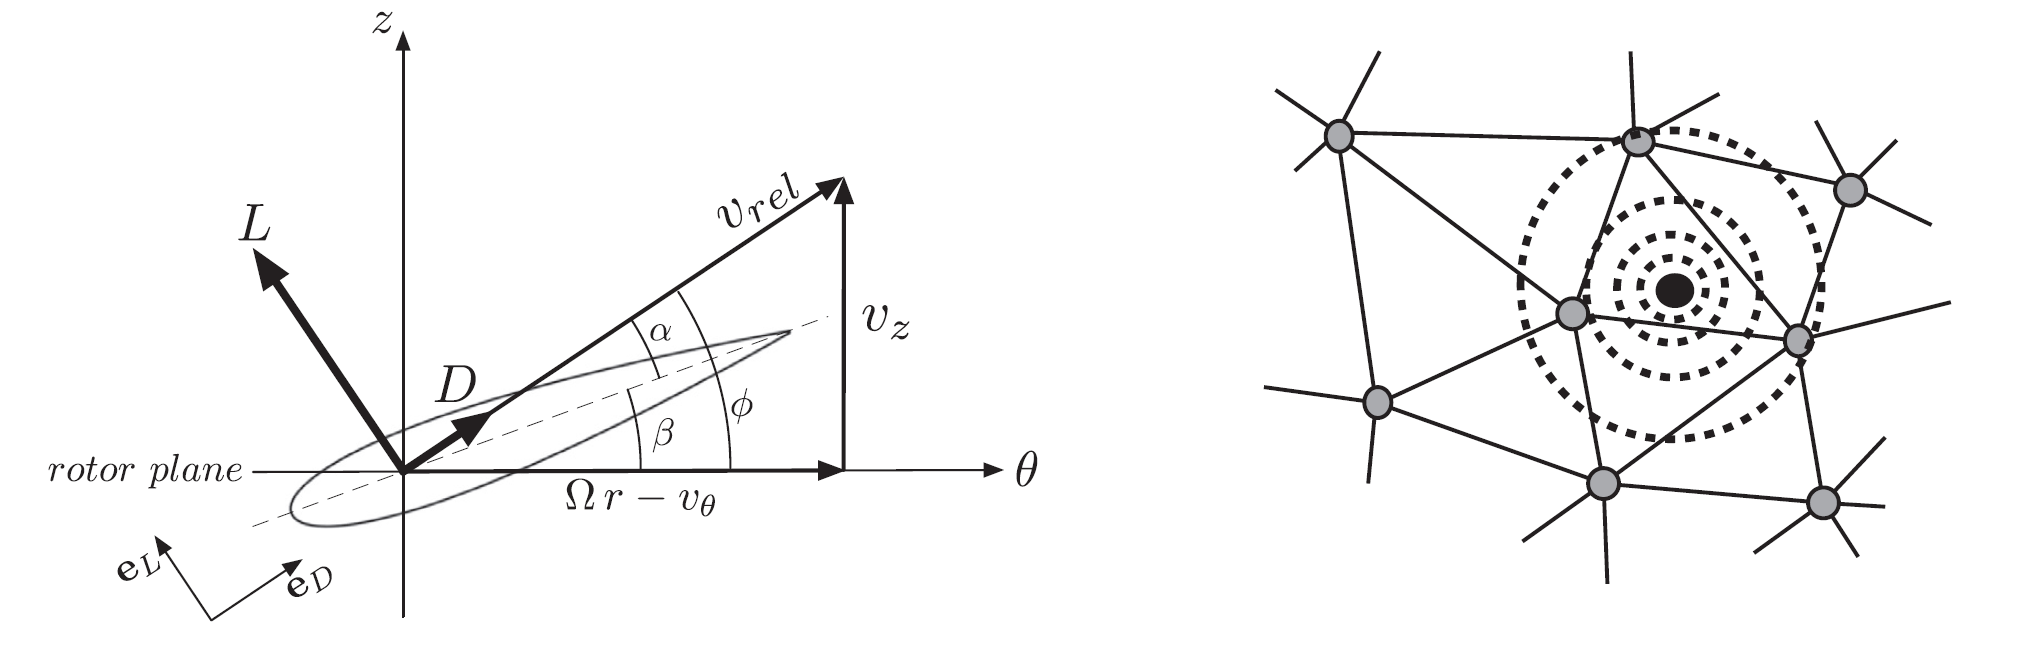
\includegraphics[scale=0.4]{./part2_developments/figures_ch4_SLI/ALM_airfoil_and_mollification_benard}
	\caption[ALM illustration of a velocity triangle and geometrical conventions in an airfoil and mollification of a point force on several nodes of an unstructured grid]{ALM illustration of a velocity triangle and geometrical conventions in an airfoil (\textsl{left}) and mollification of a point force on several nodes of an unstructured grid (\textsl{right}). Source: \citeColor[benard_large-eddy_2018].}
	\label{fig:ALM_airfoil_and_mollification_benard}
\end{figure} 
 

In the computational domain, the body forces cannot be directly applied in a single point since it would create a numerical singularity in the Navier-Stokes equations. Therefore, the body source term is applied using a mollifying function $\eta$ that distributes the body force $f$ from the forces calculated at each blade element:

\begin{equation}
\textbf{f} \left( \textbf{x}, t \right) = - \sum_{e=1}^{N} \left( L \textbf{e}_L + D \textbf{e}_D \right) \eta \left( |\textbf{r} - \textbf{r}_e| \right)
\end{equation}

where $\textbf{e}_L$ and $\textbf{e}_D$ are the unit vectors along the lift and drag directions (Figure \ref{fig:ALM_airfoil_and_mollification_benard} left), the subscript $e$ refers to each blade element and the mollifying function is defined by Eq. (\ref{eq:ch4_ALM_mollification_function}).

\begin{equation}
\label{eq:ch4_ALM_mollification_function}
\eta \left( d \right) = \frac{1}{\epsilon^3 \pi^{3/2}} \exp \left[ - \left( \frac{d}{\epsilon} \right)^2 \right]
\end{equation}

where $\epsilon = 2 w$. The mollification process is depicted in Figure \ref{fig:ALM_airfoil_and_mollification_benard} right. The simplicity of ALM and its applicability to represent the perturbations created by solid blades have seen its application to model the interaction with other bodies, such as towers in wind turbines \citeColor[benard_large-eddy_2018], and to use it for generating synthetic turbulence in the grids \citepColor[houtin-mongrolle_actuator_2020]).

%As shown in Figure (\textbf{Ref. to figure in introduction}), the dense core has a perturbation effect towards the gas phase. The resulting vortical structures will influence the dispersion of the droplets generated by atomization due to turbulent interaction. Therefore,


\subsection{Dense core representation as an actuator}

%In this work, ALM is used to model the perturbation effect of the JICF dense core on the gaseous field in dispersed phase simulations. 

As depicted in Figure \ref{fig:arienti_2006_jicf}, the presence of the dense core creates a wake and vortical structures further downstream. This interaction can be captured in resolved atomization simulations (see $\S$\ref{subsec:ch5_dense_core_in_ACLS_simus} of Chapter \ref{ch5:jicf_resolved_simulations}), but not in dispersed phase simulations where the coherent liquid structures are neglected. Since these liquid-gas interactions can have a strong influence on the transport of droplets in the developed spray region, it is of interest to model this effect in dispersed phase simulations. For this purpose, ALM is used.

\begin{figure}[h!]	
	\centering
	\includeinkscape[inkscapelatex=false,width=13cm]{./part2_developments/figures_ch4_SLI/ALM_DC_learning}
	\caption[Representation of the dense core as an actuator]{Representation of the dense core as an actuator, showing lateral (\textsl{left}) and frontal (\textsl{right}) views of the jets. \textsl{Top}: schematic dense core from a resolved simulation. \textsl{Bottom}: actuator line model of the dense core.}
	\label{fig:ALM_DC_learning}
\end{figure}

Figure \ref{fig:ALM_DC_learning} shows the representation of the dense core (top figures) as an actuator line model (bottom figures). Its complex topology is emulated by a frustum with increasing chord from the bottom ($c_0 = d_\mathrm{inj}$) to the top ($c_L = W$). The frustum has a length $L$ and an inclination angle $\theta$ which are obtained from the breakup point coordinates $(x_b, z_b)$ of the dense core in resolved atomization simulations: $L = \sqrt{x_b^2 + z_b^2}$ and $\theta = \tan^{-1} \left( z_b / x_b\right)$. The actuator points where discrete forces are placed are equally-spaced with a distance $w$ along the center line of the frustum. The number of points $N_p$ also needs to be specified in the ALM model.

Apart from the geometry, the forces applied to the actuator points are also defined. In this model, instead of specifying coefficients as done in wind turbine blades, the forces will be directly imposed in the actuator points. As shown in Figure \ref{fig:ALM_DC_learning}c, the force in the actuator will evolve linearly from the bottom to the top in order to take into account the real increasing cross-section of the actuator, which has the effect of increasing drag \citepColor[mashayek_jet_2006]. The force acts in a direction normal to the axis of the frustum. Therefore, the imposed forces can be decomposed into two components: a drag force $D$ along the $x$ direction and a lift force $L$ along the $z$ direction. Forces are specified at each actuator point with coordinates $\left( x_p, z_p \right)$ along the actuator. As the coordinates are automatically calculated according to the number of actuator points $N_p$ and the breakup point $\left( x_b, z_b \right)$, the forces will be expressed with respect to the line coordinate $s_p = \left( x_p^2 + z_p^2 \right)^{1/2}$ with expresses the distance of each actuator point to its base. Hence, the force decomposition into lift and drag holds as follows:

\begin{equation}
\textbf{F} \left( s_p \right) = D \left( s_p \right) \textbf{i} + L \left( s_p \right) \textbf{k} 
\end{equation}

where $\textbf{i}$ and $\textbf{k}$ are the unit vectors in the $x$ and $z$ directions, respectively. To estimate these forces, the net force applied to the dense core $\textbf{F}_\mathrm{DC}$ is obtained from the resolved simulations (see $\S$\ref{subsec:ch4_ALM_forces_determination}). This force is assumed to act in the same direction as the forces $\textbf{F} \left( s_p \right)$ from the actuator model, and is repartitioned into the several forces that are applied to the actuator points. Therefore, the following condition must be fulfilled:

\begin{equation}
\sum_{p=1}^{N_p} | \textbf{F} \left( s_p \right)| = | \textbf{F}_\mathrm{DC} |
\end{equation}

As the forces $| \textbf{F} \left( s_p \right)|$ increase linearly along the actuator, its evolution is represented by the following expression accordingly to the vertical coordinates $z_p$ of the actuator points:

\begin{equation}
|\textbf{F} \left( s_p \right) | = | \textbf{F}_\mathrm{DC} | \frac{s_p}{\sum_{p=1}^{N_p} s_p}
\end{equation}

And finally, the drag and lift forces to impose are calculated as follows:

\begin{subequations}
\label{eq:ALM_SLI_lift_drag_definitions}
\begin{align}
L \left( s_p \right) &= - |\textbf{F} \left( s_p \right) | \cos \theta = - | \textbf{F}_\mathrm{DC} | \cos \theta \frac{s_p}{\sum_{p=1}^{N_p} s_p} \\
D \left( s_p \right) &= |\textbf{F} \left( s_p \right) | \sin \theta = | \textbf{F}_\mathrm{DC} | \sin \theta \frac{s_p}{\sum_{p=1}^{N_p} s_p}
\end{align}
\end{subequations}

Therefore, the forces imposed to the actuator points are parametrized by the dense core net force $| \textbf{F}_\mathrm{DC} |$, the actuator inclination $\theta$ and the actuator points. Table \ref{tab:alm_parameters} shows a recap of the parameters used in the proposed model. In this table, the angle $\theta$ is not shown since it can be obtained with trigonometry from the initial and end points of the actuator. The number of actuator points $N_p$ is not taken as an input parameter as it has been checked that, if large enough, it does not have an effect of the perturbed flow field: therefore, it has been set to $N_p = 100$ for all cases presented in this thesis.

%The actuator chords shown in Figure \ref{fig:ALM_DC_learning} are not shown in this model since the increase in cross-section is directly contained in the linear evolution of the forces, Eqs. (\ref{eq:ALM_lift_drag_definitions}).

\begin{table}[!h]
\centering
\caption{Parameters of an actuator representing the dense core}
\begin{tabular}{ccc}
\thickhline
\textbf{Parameter} & \textbf{Units} & \textbf{Description} \\ 
\thickhline
$x_b, z_b$ & mm & Actuator end point  \\
%$c_0$ & mm & Chord at base of actuator \\
%$c_L$ & mm & Chord at tip of actuator \\
%$\theta$ & $\degree$ & Dense core inclination  \\
$| \textbf{F}_\mathrm{DC} |$ & N & Dense core net force\\
%$\Delta p$ & Pa & \\
\thickhline 
\end{tabular}
\label{tab:alm_parameters}
\end{table}


\subsection{Determination of forces}
\label{subsec:ch4_ALM_forces_determination}

The forces to impose in the actuator model are learnt from the resolved atomization simulation. For this purpose, the forces are firstly calculated in these simulations by calculating the corresponding term of the momentum equation (\ref{eq:momentum_conservation_general_integral}):

\begin{equation}
\boldsymbol{F}_\mathrm{DC} = \boldsymbol{F}_p + \boldsymbol{F}_\tau = \int_{\partial \Omega_{DC}} \left( \underbrace{- p \boldsymbol{n}}_{\mathrm{Pressure}} + \underbrace{2 \mu \overline{\overline{\epsilon}} \boldsymbol{n}}_{\mathrm{Shear}}  \right) dS 
\end{equation}

where $\partial \Omega_{DC}$ denotes the dense core surface. $\boldsymbol{F} $ has two contributions: a pressure force term and a shear force term. In a first instance, the shear term is neglected (see next section for details). Therefore, the total force term is reduced to the pressure force:

\begin{equation}
\label{eq:ALM_Fp_complete_integral}
\boldsymbol{F}_\mathrm{DC} = \boldsymbol{F}_p = - \int_{\partial \Omega_{DC}} p \boldsymbol{n} dS 
\end{equation}

To simplify this expression, the forces in the windward and leeward sides of the dense core are assumed to be constant as indicated in Figure \ref{fig:ALM_DC_learning}a by the red and blue arrows, respectively. The surface of the dense core can be approximated according to the actuator model as $\partial \Omega_\mathrm{DC} \approx S_\mathrm{DC} = \frac{1}{2} \left( c_0 + c_L \right) L$, being $L = \sqrt{x_\mathrm{b}^2+z_\mathrm{b}^2}$ if the actuator initial point is located at the origin of the coordinate system. Therefore, Eq. (\ref{eq:ALM_Fp_complete_integral}) can be reduced to


\begin{equation}
\label{eq:ALM_Fp_calculation_simplified}
\boxed{
|\boldsymbol{F}_\mathrm{DC}| = \left( p_\mathrm{windward} - p_\mathrm{leeward} \right) S_{DC} 
}
\end{equation}


%The approximation of considering the pressures as both sides as equal is done in this model as it has been observed in the resolved simulations (see Figure \textbf{????}), but requires further research and might be a source of error. 

It must be taken into account that the dense core as a rigid body immersed in a fluid. Its geometry has been approximated by observations of the dense core shape in resolved atomization simulations, and have been taken as constant. In reality, the dense core is a deformable body whose topology (breakup point, inclination, length) changes with time. Future works on deriving more thorough models intending to represent the dense core should take into account these transient properties \citepColor[patil_liquid_2021].

\subsubsection*{Neglecting the shear force term}

For a body immersed in a fluid, the shear force is defined as:

\begin{equation}
\boldsymbol{F}_\tau = \int_{\partial \Omega_\mathrm{DC}} 2 \mu \overline{\overline{\epsilon}} \boldsymbol{n} dS
\end{equation}

where $\overline{\overline{\epsilon}}$ is the deformation tensor:

\begin{equation}
\overline{\overline{\epsilon}} = \frac{1}{2} \left( \nabla \boldsymbol{u} + \left(\nabla \boldsymbol{u}\right)^T \right)
\end{equation}

The forces $\boldsymbol{F}_\tau$ cannot be easily calculated with the current methodology. Instead, a more simple expression of the shear forces based on a friction coefficient $C_f$ and a reference surface $S$ is used \citemColor[johnston_investigation_1984,soedarmo_simplified_2018]:

\begin{equation}
\label{eq:ALM_model_Ftau}
\boldsymbol{F}_\tau = \frac{1}{2} \rho_g u_g^2 S C_f 
\end{equation}

The friction coefficient $C_f$ is obtained from the following expression \citepColor[yang_new_2017]:

\begin{equation}
\label{eq:ALM_model_Cf}
C_f = 0.37 \left( \log Re_x \right)^{-2.584}
\end{equation}

where $Re_x$ is the Reynolds number based on the incoming velocity and the distance along the dense core.


The relative intensity of the force $\boldsymbol{F}_p$ with respect to $\boldsymbol{F}_\tau$ can be measured by dividing expressions (\ref{eq:ALM_Fp_complete_integral}) and (\ref{eq:ALM_model_Ftau}), plugging also Eq. (\ref{eq:ALM_model_Cf}):

\begin{equation}
\label{eq:rF_definition}
r_F = \frac{| \boldsymbol{F}_p| }{| \boldsymbol{F}_\tau |} = \frac{\Delta p}{0.185 \rho_g u_g^2 \left( \log Re_x \right)^{-2.584}}
\end{equation}


Where $\Delta p \sim O \left( 10^4 \right) $ in the operating points studied (see Table \ref{tab:jicf_operating_conditions} and Figure \ref{fig:JICF_turbulent_structures_planes_x} from Chapter \ref{ch5:jicf_resolved_simulations}). Considering this value, the expression for $r_F$ can be estimated to be:

\begin{equation}
r_F \sim \frac{10^5}{\rho_g u_g^2 \left( \log Re_x \right)^{-2.584}}
\end{equation}

According to the operating points studied (see Chapter \ref{ch5:jicf_resolved_simulations}), the values of $Re_x$ range from $10^3$ to $10^5$. In such points, $\rho_g = 7.21$ kg m$^{-3}$ and $u_g = 75; 100$ m s$^{-1}$. With these values, the expression of $r_F$ can be plotted as a function of $Re_x$ in Figure \ref{fig:ALM_rF_vs_Rex}. As observed, the ratio $r_F$ presents values between 10 to 90 for the $Re_x$ range of interest. These ratios mean that the pressure force $\boldsymbol{F}_p$ is between 10 and 90 times the shear force $\boldsymbol{F}_\tau$. Therefore, $|\boldsymbol{F}_\tau| << |\boldsymbol{F}_p|$ and only the contribution of the pressure force is considered to calculate the dense core net force.




\begin{figure}[h!]
	\centering
	\includegraphics[scale=0.5]{./part2_developments/figures_ch4_SLI/ALM_rF_vs_Rex.eps}
	\caption{Force ratio evolution with $Re_x$.}
	\label{fig:ALM_rF_vs_Rex}
\end{figure}


\section{Secondary atomization modeling}
\label{sec:ch4_secondary_atomization_modeling}

In disperse phase simulations, spray is modeled by a set of spherical and rigid particles whose dynamics are governed by the point-particle equations described in $\S$\ref{sec:ch3_EL_formalisms}. Due to these assumptions, particles will not break by their interaction with the gaseous phase as in the resolved atomization simulations. Nevertheless, further breakup can be taken into account by means of secondary atomization models. The most important parameter governing secondary atomization is the Weber number based on the relative velocities between liquid and gas $u_\mathrm{rel}$:

\begin{equation}
\label{eq:We_secondary_atomization_definition}
We = \frac{\rho_g u_\mathrm{rel}^2 r}{\sigma} 
\end{equation}

Different mechanisms produce secondary atomization depending on the value of We, see Fig. \ref{fig:regimes_atomization_secondary}. Existing models for secondary atomization have been developed for each particular mode of breakup, such as the WAVE model for high Weber numbers \citepColor[reitz_modeling_1987] or the Taylor Analogy Breakup (TAB) model for low ones \citepColor[orourke_tab_1987]. The former model predicts breakup by following a linear stability analysis considering Kelvin-Helmholtz waves as the governing breakup mechanisms, while the latter makes an analogy between a droplet and a second-order mechanical system. Nevertheless, up to date there is not a model which accounts for all different breakup mechanisms and that can capture all the physical complexity of secondary atomization.

In this work, three atomization models have been implemented and tested: the TAB model, the Enhanced TAB model \citepColor[tanner_liquid_1997], and the stochastic model of \citeColor[gorokhovski_stochastic_2001]. They are described in the following sections.

\subsection{Taylor Analogy Breakup}


\begin{figure}[h!]
	\centering
	\includeinkscape[inkscapelatex=false,scale=0.75]{./part2_developments/figures_ch4_SLI/TAB_analogy}
	\caption{Taylor analogy breakup between a droplet and a mechanical system with spring and damper. The undeformed droplet is represented by the dashed line, while the thick solid line depicts the droplet after deformation. $x$ is the displacement from the deformed to the undeformed states.}
	\label{fig:TAB_droplet_deformation}
\end{figure}

The Taylor Analogy Breakup (TAB) model is one the first secondary atomization models. Developed by \citeColor[orourke_tab_1987], it makes an analogy between a droplet and a mechanical system as shown in Fig. \ref{fig:TAB_droplet_deformation}. Breakup occurrence is estimated by solving the ordinary differential equation (ODE) representing the oscillating dynamics of the mechanical system depicted:

\begin{equation}
\label{eq:TAB_ODE_x}
m \ddot{x} = F - k x - c \dot{x}
\end{equation}

where $x$ is the displacement from the droplet's equator due to deformation, $m$ is the mass, $F$ is the external force, $k$ is the spring constant and $c$ is the damping coefficient. The Taylor analogy makes a comparison between this mechanical system and the droplet, producing the following relation between constants:

\begin{equation}
\frac{F}{m} = C_F \frac{\rho_g u_\mathrm{rel}^2}{\rho_l r} ~~~~ ; ~~~~ \frac{k}{m} = C_k \frac{\sigma}{\rho_l r^3} ~~~~ ; ~~~~ \frac{c}{m} = C_d \frac{\mu_l}{\mu_g r^2}
\end{equation}

where $C_F = 1/3$, $C_k = 8$, $C_d = 5$ are constants, $r$ the droplet radius, $\rho$ the density, $\sigma$ the surface tension, $\mu$ the viscosity, and the subscripts $l$ and $g$ indicate liquid and gases respectively. 

The deformation $x$ can be expressed by a non-dimensionless parameter $y$, hereafter referred as droplet distorsion, whose equivalence is $y = x / \left( C_b r \right)$, where $C_b = 0.5$ is a constant. Using the expressions from the Taylor analogy and introducing the change of variable $y$, the ODE (\ref{eq:TAB_ODE_x}) changes to:

\begin{equation}
\label{eq:TAB_ODE}
\ddot{y} = \frac{C_F}{C_b} \frac{\rho_g}{\rho_l} \frac{u_{rel}^2}{r^2} - \frac{C_k \sigma}{\rho_l r^3} y - \frac{C_d \mu_l}{\rho_l r^2} \dot{y}
\end{equation}

This expression governs the breakup of droplets, which occurs for $y > 1$ (i.e. when the amplitude of the oscillation $x$ equals the radius of the undeformed droplet). For solving this equation, it is useful to introduce the following parameters:

\begin{subequations}
\label{eq:TAB_td_omega_definition}
\begin{align}
t_d &= \frac{2 \rho_l r^2}{C_d \mu_l} \\
\omega^2 &= C_k \frac{\sigma}{\rho_l r^3} - \frac{1}{t_d^2}
\end{align}
\end{subequations}

where $t_d$ is the oscillation damping time and $\omega$ is the oscillations frequency. With these definitions, the solution to Eq. (\ref{eq:TAB_ODE}) is:

\begin{equation}
\label{eq:yTAB_equation_general}
y \left( t \right) = We_c + e^{- t / t_d} \left[ \left( y_0 - We_c \right) \cos \left( \omega t \right) + \frac{1}{\omega}\left( \dot{y}_0 + \frac{y_0 - We_c}{t_d} \right) \sin \left( \omega t \right)   \right]
\end{equation}

where $We_c = \frac{C_F}{C_k C_b} We = We / 12$ with the constants previously defined. The distorsion rate can be obtained by differentiating the former expression with time:

\begin{equation}
\label{eq:dydtTAB_equation_general}
\dot{y} \left( t \right) = \frac{We_c - y \left( t \right) }{t_d} + e^{- t / t_d} \left[ \left( \dot{y}_0 + \frac{y_0 - We_c}{t_d} \right) \cos \left( \omega t \right) - \omega \left( y_0 - We_c \right) \sin \left( \omega t \right)  \right]
\end{equation}

As it can be seen, the previous equations are continuous. For numerical implementation of the algorithm, it is more convenient to express them in their corresponding discrete form:

\begin{equation}
\label{eq:yTAB_equation_discrete}
y^{n+1} = We_c + e^{- dt / t_d} \left[ \left( y^n - We_c \right) \cos \left( \omega dt \right) + \frac{1}{\omega}\left( \dot{y}^n + \frac{y^n - We_c}{t_d} \right) \sin \left( \omega dt \right)   \right]
\end{equation}

\begin{equation}
\label{eq:dydtTAB_equation_discrete}
\dot{y}^{n+1} = \frac{We_c - y^{n+1} }{t_d} + e^{- dt / t_d} \left[ \left( \dot{y}^n + \frac{y^n - We_c}{t_d} \right) \cos \left( \omega dt \right) - \omega \left( y^n - We_c \right) \sin \left( \omega dt \right)  \right]
\end{equation}

where the subindexes $n$ and $n+1$ indicate two consecutive time instants separated by the timestep $dt$.

To estimate breakup, firstly $\omega^2$ is calculated with Eq. (\ref{eq:TAB_td_omega_definition}b). According to its value, two scenarios are possible:

\begin{itemize}

	\item If $\omega^2 < 0$, oscillations are not present. Hence, the droplet does not deform and the values for droplets distorsion and distorsion rate are set to $0$: $y^{n+1} = y^n = 0$.
	
	\item If $\omega^2 > 0$, breakup is possible. In this case, the amplitude of oscillations $A$ is calculated:
	
	\begin{equation}
	A = \sqrt{\left( y^n - We_c \right)^2 + \left( \dot{y}^n / \omega \right)^2}
	\end{equation}

\end{itemize}

Again, the value of $A$ will present two different alternatives:

\begin{itemize}

	\item If $We_c + A \leq 1$, then $y^n \leq 1$ and droplet will not break. Deformation and deformation rate will then be updated by applying Eqs. (\ref{eq:yTAB_equation_discrete}) and (\ref{eq:dydtTAB_equation_discrete}).
	
	\item If $We_c + A > 1$, breakup is possible. A breakup timestep $dt_{bu}$ is then calculated as the smallest root of the following equation:
	
	\begin{equation}
	\label{eq:TAB_dtbu_obtention}
	We_c + A \cos \left( \omega dt_{bu} + \phi  \right) = 1
	\end{equation}

\end{itemize}

where the phase $\phi$ is obtained from the following:

\begin{equation}
\cos \phi = \frac{\dot{y}^n - We_c}{A} ~~~~ ; ~~~~ \sin \phi = - \frac{\dot{y}^n}{A \omega}
\end{equation}

Breakup will then occur in the case that $dt < dt_{bu}$, or also if updating the deformation it is found that $y^{n+1} > 1$. Once breakup is triggered, the associated droplet (named parent) will divide into one or several smaller particles (named children). The mean size of children droplets $r_{32}$ is obtained through an energy balance between the produced droplets and the parent with radius $r$, yielding the following relation between both sizes:

\begin{equation}
\label{eq:TAB_model_radius_ratio}
\frac{r}{r_{32}} = 1 + \frac{8 K}{20} + \frac{\rho_l r^3}{\sigma} \dot{y}^2 \left( \frac{6 K - 5}{120} \right)
\end{equation}

where $K = 10/3$ is a constant. Now, radii of children droplets $r_{ch}$ are randomly chosen from a Rosin-Rammler distribution \footnote{In the original work by \citeColor[orourke_tab_1987], a $\chi^2$ distribution is used} with characteristic diameter $r_{32}$ and factor $q = 3.5$: 


\begin{equation}
\label{eq:rossin_rammler_distribution}
Q \left( r \right) = 1 - \exp\left(  - \left( \frac{r}{r_{0.632}} \right)^q \right)
\end{equation}

which can be inverted to obtain $r_{ch}$:

\begin{equation}
\label{eq:r_ch_TAB_family}
r_{ch} = r_{32} \sqrt[3.5]{- \log \left( 1 - Q \right) }
\end{equation}

where $Q$ is Cumulative Density Function (CDF). To estimate the size of children droplets droplets from this distribution, $Q$ is randomly sampled from a uniform distribution $\in [0,1]$. The resulting random number is introduced in the previous expression, yielding a value for one children droplet. This procedure is repeated until the volume of all children droplets equals the volume of the parent, hence conserving mass. Children droplets are then randomly located along the surface of the parent droplet. They will all inherit the velocity of the parent droplet, plus a component $v_\perp$ with magnitude:

\begin{equation}
\label{eq:TAB_v_perp}
v_\perp = C_v C_b r \dot{y}^n
\end{equation}

where $C_v \approx 1$. The direction of $v_\perp$ is randomly chosen in a plane normal to the relative velocity $u_\mathrm{rel}$. Finally, all children droplets all initialised with $y = \dot{y} = 0$.



\subsection{Enhanced TAB model}

The main disadvantage of the TAB model is the underprediction of droplets size. To overcome this problem, an improved version of the TAB model was developed by \citeColor[tanner_liquid_1997], named Enhanced Taylor-Analogy Breakup (ETAB). Breakup is predicted and triggered in the same way as in TAB, but the size of children droplet is estimated differently. While TAB makes use of an energy balance \citepColor[orourke_tab_1987], ETAB considers that the droplet production rate is proportional to the number of children droplets. Mathematically, this proportionality is expressed by the following exponential decay law:

\begin{equation}
\label{eq:ETAB_rate_production_law}
\frac{d m_\mathrm{ch}}{dt} = - 3 K_\mathrm{br} m_\mathrm{ch}
\end{equation}

where $m_\mathrm{ch}$ is the mass of children droplets. This law depends on the atomization regime through the breakup constant $K_\mathrm{br}$, which depends on $We$ and the oscillation frequency $\omega$:

\begin{equation}
\label{eq:ETAB_Kbr_equation}
K_{br} =
\left\{
    \begin{split}
    k_1 \omega \,\,\mathrm{if}\,\,We \leq We_t \\ 
    k_2 \omega \sqrt{We} \,\,\mathrm{if}\,\,We > We_t
    \end{split}
\right.
\end{equation}

where $k_1$ and $k_2$ are constants, and $We_t$ is a transition Weber number between bag and stripping breakup regimes, set to 80 \citepColor[tanner_liquid_1997]. The bag breakup $k_1$ is obtained from the following expression to make a smooth transition between both regimes:

\begin{equation}
k_1 = k_1^* \left[\left(  \frac{k_2}{k_1^*} \left( \sqrt{We_t} - 1 \right) \right) \left( \frac{We}{We_t} \right)^4 + 1 \right]
\end{equation}

where $k_1^* = 2/9$. The stripping breakup constant is fixed to $k_2 = 2/9$.

The size of children droplets is calculated by integrating the production law Eq. (\ref{eq:ETAB_rate_production_law}):

\begin{equation}
\label{eq:ETAB_model_radius_ratio}
\frac{r_{ch}}{r} = e ^{-K_{br} t_{bu}}
\end{equation}

where $t_{bu}$ is estimated as in the TAB model, Eq. (\ref{eq:TAB_dtbu_obtention}). All children droplets generated from a parent with radius $r$ will have identical size $r_{ch}$. Finally, children will inherit parent's velocity plus a normal component given by:

\begin{equation}
v_\perp = C_A C_b r \left(\dot{y}^n\right)^2 
\end{equation}

whose direction is randomly chosen in a plane normal to the relative velocity $u_\mathrm{rel}$. In this expression, $C_A$ is a constant determined from an energy balance:

\begin{equation}
C_A^2 = 3 \left( 1 - \frac{r_{ch}}{r} + \frac{5}{72} C_D We \right) \frac{\omega^2}{\dot{y}^2}
\end{equation}

being $C_D$ is the drag coefficient of the parent droplet, Eq. (\ref{eq:Re_CD_droplet}). Note that $v_\perp$ defined by the ETAB model differs from TAB's Eq. (\ref{eq:TAB_v_perp}) by considering $C_A$ to be dependent on the breakup regime.


\subsection{Gorokhovski stochastic model}
\label{subsec:ch4_goro_model}

Both TAB and ETAB models were derived using the Taylor analogy breakup. The TAB model is known \citemColor[tanner_liquid_1997,dahms_significance_2016,fontes_improved_2019] to underestimate the diameter of the children droplets and to not distinguish between breakup regimes,
producing too many droplets when the Weber number is high. Hence, the applicability of TAB is restricted to breakup at low $We$. ETAB tried to solve this issue by considering an exponential decay law for the size of children droplets which would depend on the breakup regime. Both models are, however, deterministic in the sense that a single range of droplet sizes is considered when breakup is produced.

A different secondary atomization model not based on the Taylor analogy was derived by \citeColor[gorokhovski_stochastic_2001]. This model circumvents the deterministic approach of the TAB family of models by accounting for a range of children droplet sizes when breakup occurs. This is done by using a stochastic approach based on Kolmogorov's theory of breakup \citepColor[kolmogorov_log-normal_1941]. Following this theory, the evolution of droplet's sizes is represented by a Fokker-Planck equation: 

\begin{equation}
\frac{\partial T \left( \ln r, t \right)}{\partial t} = - \nu  \langle \xi \rangle  \frac{\partial T \left( \ln r, t \right)}{\partial \left( \ln r \right)} + \frac{1}{2} \nu  \langle \xi^2 \rangle  \frac{\partial^2 T \left( \ln r, t \right)}{\partial \left( \ln r \right)^2}
\end{equation}

where $T \left( \ln r, t \right)$ is the cumulative distribution of droplets sizes, $\nu$ the breakup frequency, and  $\langle \xi \rangle$ and $ \langle \xi^2 \rangle$ are parameters. After some mathematical development \citepColor[apte_les_2003], the cumulative distribution function can be expressed as:

\begin{equation}
\label{eq:gorokhovski_T_CDF}
T \left( \ln r, t \right) = \frac{1}{2} \left( 1 + \erf \left( \frac{\ln r - \ln r_{ch} - \langle \xi \rangle }{\sqrt{2 \langle \xi^2 \rangle}}\right)  \right)
\end{equation}

This function will be later used to obtain the size of children droplets. The previous step is to determine when breakup occurs. In this model, two criteria are used:

\begin{itemize}

	\item Parent droplets must be larger than a critical radius $r_\mathrm{cr}$. This value is determined from a critical Weber number $We_\mathrm{crit} = 6$:
	
	\begin{equation}
	r_\mathrm{crit} = \frac{We_\mathrm{crit} \sigma}{\rho_g u_\mathrm{rel}^2}
	\end{equation}
	
	\item The residence time of the particles must be larger than a computed breakup time $t_\mathrm{bu}$:
	
	\begin{equation}
	t_{bu} = B \sqrt{\frac{\rho_l}{\rho_g}} \frac{r}{u_{rel}}
	\end{equation}
	
	where $B = \sqrt{3}$.

\end{itemize}

If both $r > r_\mathrm{crit}$ \textbf{and} $t > t_{bu}$, breakup occurs. In this case, size of children droplet is obtained from the cumulative density function $T \left( \ln r_{ch}, t \right)$, Eq. (\ref{eq:gorokhovski_T_CDF}), from which $\ln r_{ch}$ can be solved:
 
 
\begin{equation}
\label{eq:r_ch_goro}
r_{ch} = r \exp \left( \langle \xi \rangle  + \sqrt{2 \langle \xi^2 \rangle} \erf^{-1} \left(  2 T - 1 \right) \right)
\end{equation}

%\begin{equation}
%\ln r_{ch} = \ln r + \langle \xi \rangle  + \sqrt{2 \langle \xi^2 \rangle} \erf^{-1} \left(  2 T - 1 \right)
%\end{equation}

The size of children droplets are then obtained by sampling a random value of $T$ from a uniform distribution between $0$ and $1$, $T \sim \mathcal{U} \left( 0, 1 \right)$ , and then applying the previous equation. The parameters $\langle \xi \rangle$ and $\langle \xi^2 \rangle$ are calculated from the following equations:

\begin{subequations}
\label{eq:gorokhovski_epsilon_parameters_definition}
\begin{align}
\langle \xi \rangle &=  K_1 \ln \left(  \frac{We_c}{We}  \right) \\
- \frac{\langle \xi \rangle}{\langle \xi^2 \rangle} &=  K_2 \ln \left( \frac{r}{r_{crit}} \right)
\end{align}
\end{subequations}

where $K_1$ and $K_2$ are model constants, which are of order unity. The constant $K_1$ controls the mean size of children droplets, while $K_2$ influences its standard deviation.

Children droplets inherit then a velocity which has two components: the parent particle velocity in the same direction, plus a velocity normal to the parent's direction and magnitude equal to:

\begin{equation}
|\textbf{u}_\mathrm{ch,n} | = \frac{r}{t_{bu}}
\end{equation}




%
%\subsection{Analysis of sizes and number of children droplets}
%
%An analysis of sizes and estimated number of droplets produced by each model is done in the following lines.
%
%The estimated number of children for each model can be obtained as:
%
%\begin{equation}
%N_{ch} = \left( \frac{r}{r_{ch}} \right)^3
%\end{equation}
%
%\paragraph{Gorokhovski} Constants $K_1$, $K_2$ need to be tuned. \textbf{2009 Apte} uses the values $K_1 = 0.6$ and $K_2 = 1$ for simulating spray in a swirl injector. \textbf{Senoner PhD 2010} uses $K_1 = 0.1$, $K_2 = 0.8$ for simulating a diesel spray injected in a high-pressure chamber; and the values  $K_1 = 0.02$, $K_2 = 0.16$ for simulating a high-pressure jet in crossflow. The effect of these two constants will be investigated in our models.
%
%As done for the models from the TAB family, a mean size for children droplets can be estimated. The parameter $\xi$ from Eq. (\ref{eq:gorokhovski_T_CDF}) is defined as $\xi = \ln \left( \frac{r_{ch}}{r}  \right)$. Introducing this expression into Eq. (\ref{eq:gorokhovski_epsilon_parameters_definition}a) 
%
%\begin{equation}
%\langle \ln \left( \frac{r_{ch}}{r}  \right) \rangle = K_1  \ln \left(  \frac{We_c}{We}  \right) 
%\end{equation}
%
%By rearranging this equation we can express the mean size of children droplets:
%
%\begin{equation}
%\langle  \frac{r_{ch}}{r} \rangle = \left( \frac{We_c}{We} \right)^{K_1}
%\end{equation}
%
%This equation confirms the previous statement that the constant $K_1$ has a direct influence on the size of children droplet generated: the larger $K_1$ is, the smaller children droplets are (since the ratio $We_c/We < 1$). Generated children droplet can still undergo further breakup if they meet the breakup conditions (cascade effect), so decreasing $K_1$ would a priori limit the size of droplets (and hence their number) only in each iteration. Nevertheless, this can suppose a smooth transition of breakup towards equilibrium, which would ensure that the Weber number of children droplets is closer to its critical value (i.e. the limit of breakup). An aggressive breakup, which could be produced with a low value of $K_1$, could generate many children droplets from a parent particle with very small size that would not be found in reality (see Figures \ref{fig:r_ratio_gorok} and \ref{fig:N_ch_gorok}).
%
%
%
%\begin{figure}[h!]
%	\centering
%	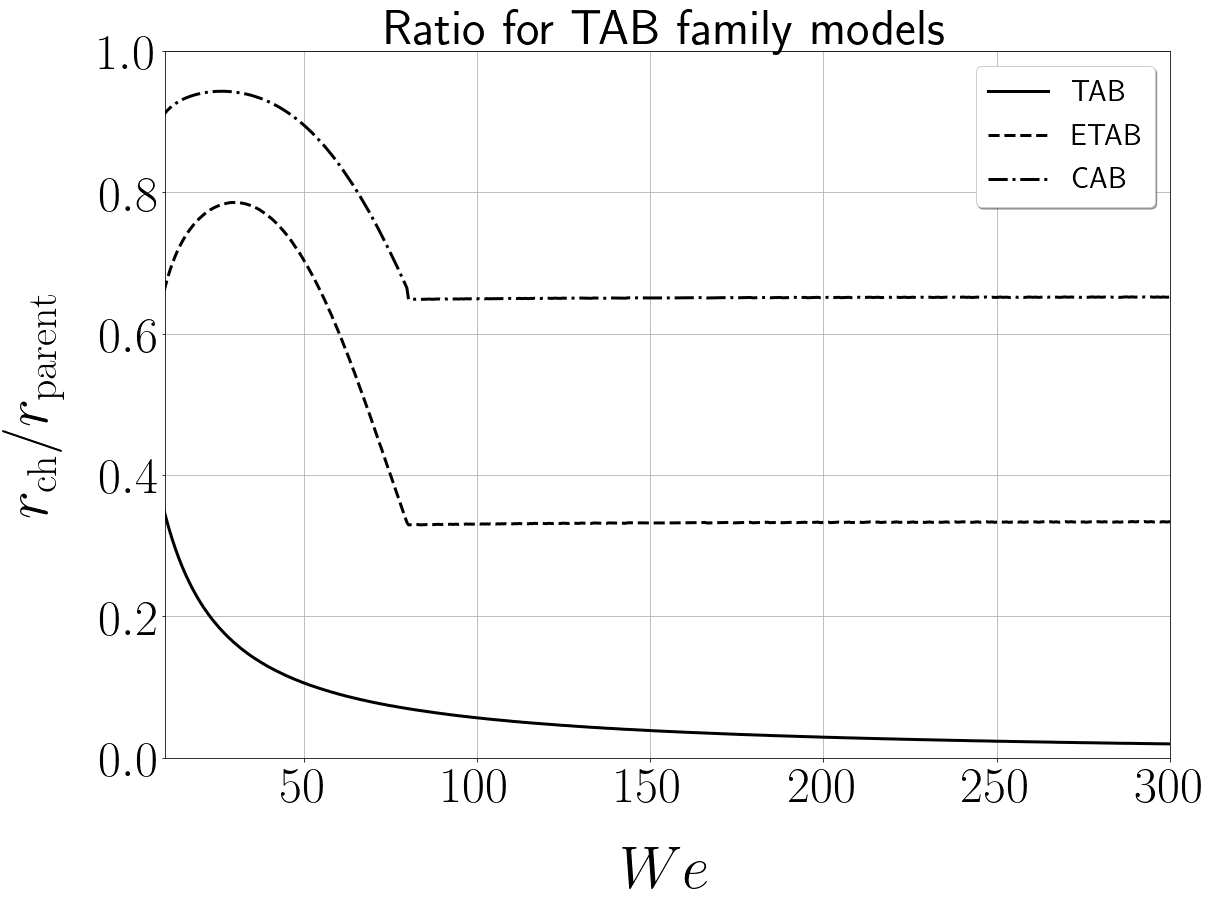
\includegraphics[scale=0.2]{./part2_developments/figures_ch4_SLI/ratio_droplet_size_TAB}
%	\caption{Ratio of mean droplet for TAB family of models}
%	\label{fig:r_ratio_TAB}
%\end{figure}
%
%\begin{figure}[h!]
%	\centering
%	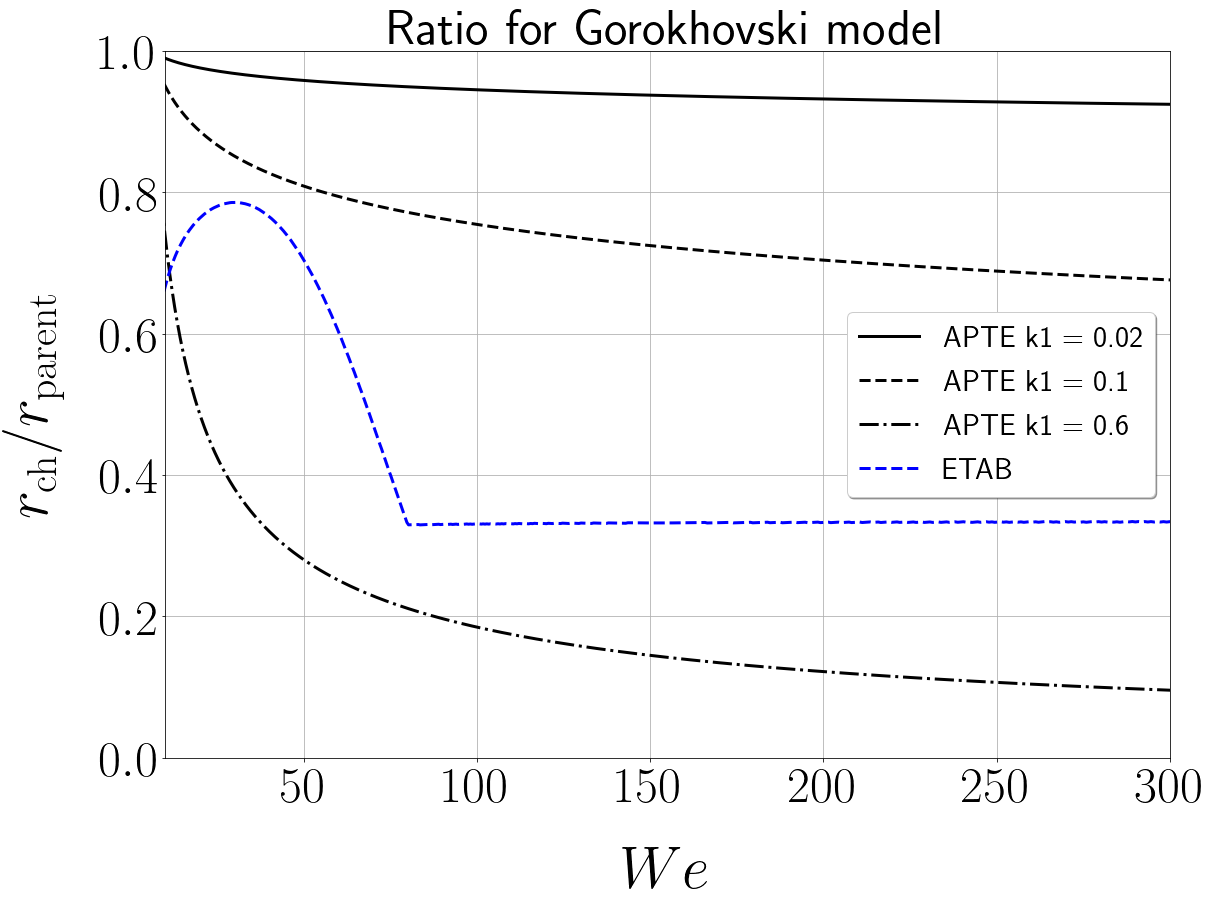
\includegraphics[scale=0.2]{./part2_developments/figures_ch4_SLI/ratio_droplet_size_gorok}
%	\caption{Ratio of mean droplet for Gorokhovski model}
%	\label{fig:r_ratio_gorok}
%\end{figure}
%
%\begin{figure}[h!]
%	\centering
%	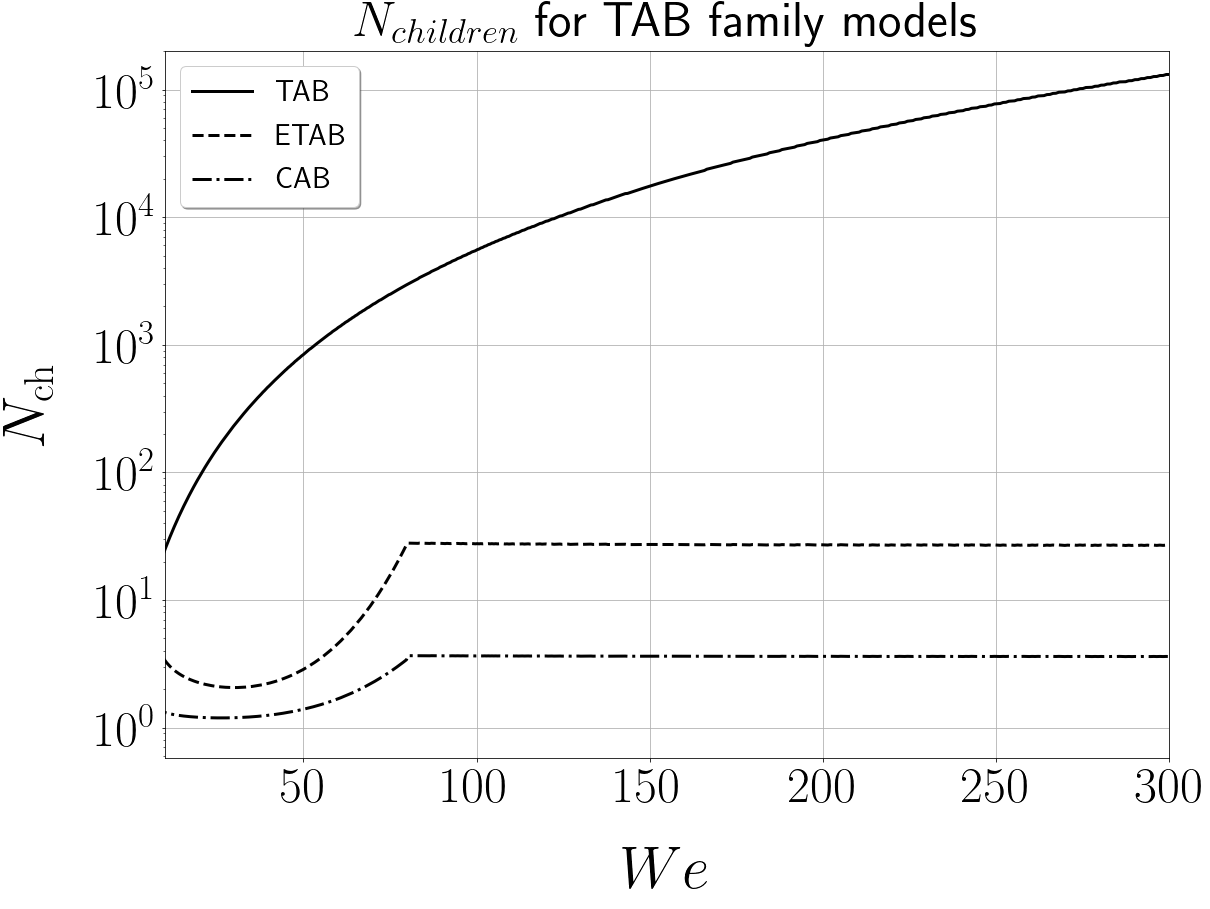
\includegraphics[scale=0.2]{./part2_developments/figures_ch4_SLI/N_ch_TAB}
%	\caption{Estimated number of children for TAB family of models}
%	\label{fig:N_ch_TAB}
%\end{figure}
%
%\begin{figure}[h!]
%	\centering
%	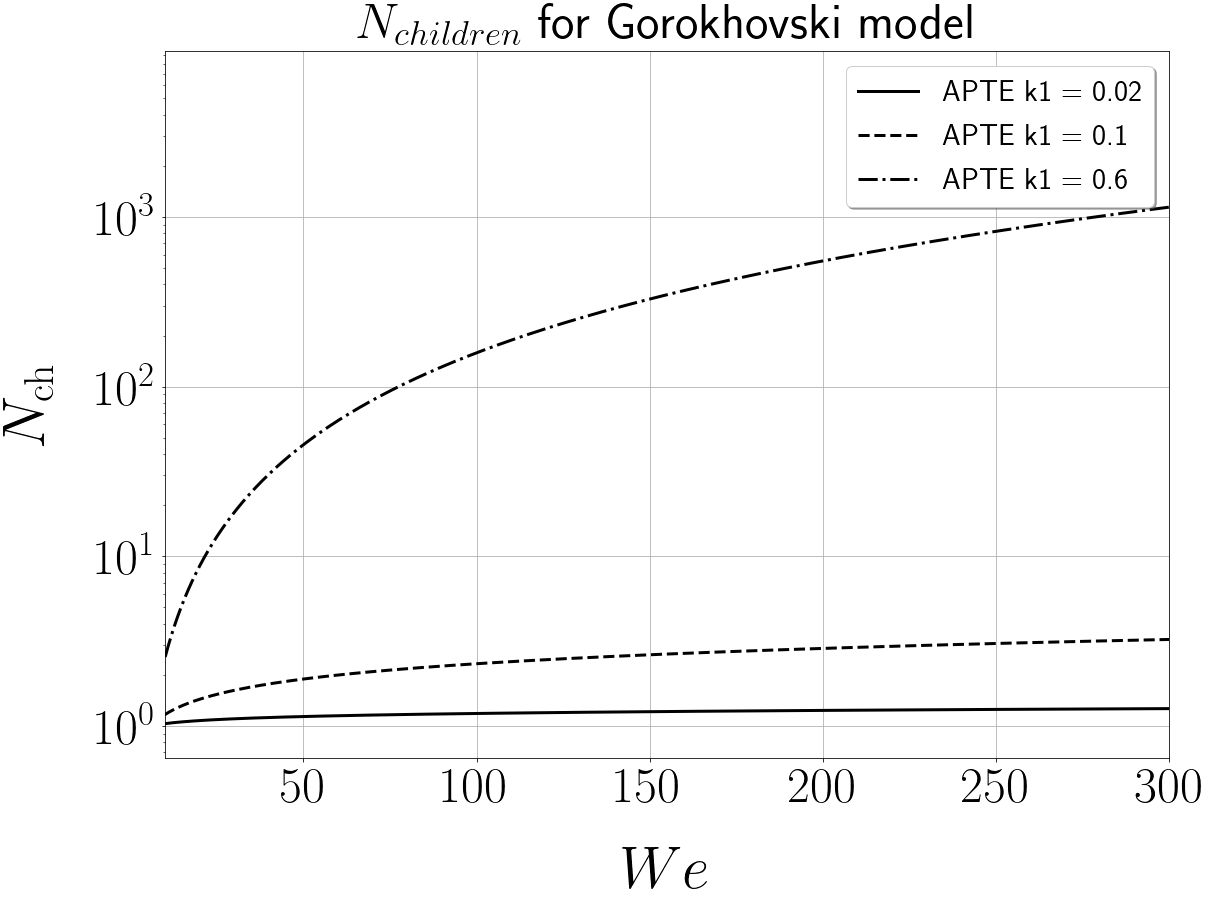
\includegraphics[scale=0.2]{./part2_developments/figures_ch4_SLI/N_ch_gorok}
%	\caption{Estimated number of children for Gorokhovski model}
%	\label{fig:N_ch_gorok}
%\end{figure}



%\section{Subgrid models for turbulent dispersion}
%
%\subsubsection*{Review}
%
%Regarding turbulent dispersion models, there are the ones used in RANS studies:
%
%\begin{itemize}
%
%	\item \textbf{2016 Eckel} mentions two dispersion models: Gosmann and Ioannides (the classic) (1983), (Blumcke et al. 1993)
%	
%	\item \textbf{Fontes 2018} uses the Langevin dispersion model introduced in Sommerfeld 2001
%
%	\item \textbf{Belmar 2020} presents a turbulent dispersion model by O'Rourke.
%
%\end{itemize}
%
%For LES, Iafrate 2016 shows a good modelling of turbulent dispersion applied to gasoline injection ($\S$8.2 Impact de la turbulence sous-maille), based on references 120-124.
%
%Also, references I have for LES are 2015 Minier, Minier ref. 57, 2014 Urzay - Particle-laden flows.
%
%A nice one is the techical report Amsden 1989 - KIVA II.
%
%OJO: reference OKongo and Bellan de Minier ref. 57 puede ser fundamental, hace analisis de particulas con distintas velocidades inyectadas !!


\section{Conclusions and perspectives}

This chapter has introduced and detailed the injection models developed in the works of this thesis. The full process is depicted by the flowchart of Figure \ref{fig:SLI_graphic_description}. The learning of the liquid injectors, baptised as SLI, is based on a spray characterization process of droplets resulting from resolved atomization simulations. Such process consists of sampling a flux-density distribution of droplets and evaluating its convergence to then make an in-plane discretization of the spray. Then, the individual sprays of the discrete grid are characterized by average values of fluxes, diameters, and velocities, and by RMS values of velocities. The spray grid can also be further refined through a convergence-driven discretization process. Then, resulting injectors can be used to inject a realistic spray in dispersed phase simulations. The models are then closed by including in the dispersed phase simulations: 1) a modelisation of the dense core perturbance effect with ALM, which is based on a learning process from the resolved atomization simulations; and 2) a secondary atomization model that continues breaking the particles in case they are not in equilibrium with the surrounding air. The next chapters are devoted to the two-phase simulations and the application of the models. \\

For further development of the models, the following perspectives could be considered:

\begin{itemize}

	\item Include a modified drag coefficient for lagrangian particles which depends on the deformation of the liquid structures sampled in resolved atomization simulations. This would allow for a more accurate transport of the lagrangian spray at the first time instants of injection, which would affect the particle's trajectories and the liquid-gas relative velocity before secondary breakup takes place. 
	
	\item Consider a transient spray obtained through the accumulation process to develop an unsteady injection model. This would be specially useful in reactive cases where thermoacoustic oscillations play an important role, such as gas turbine and rocket engines. 

	\item Extend the spray convergence criterion, defined as a MSE norm on the droplet diameters, to include other parameters such as liquid velocities.
	
	\item Improve the actuator line model developed in this thesis to make a better representation of the resolved dense core, such as by considering a transient behaviour of its topology and its force.

\end{itemize}